%Version 3 October 2023
% See section 11 of the User Manual for version history
%
%%%%%%%%%%%%%%%%%%%%%%%%%%%%%%%%%%%%%%%%%%%%%%%%%%%%%%%%%%%%%%%%%%%%%%
%%                                                                 %%
%% Please do not use \input{...} to include other tex files.       %%
%% Submit your LaTeX manuscript as one .tex document.              %%
%%                                                                 %%
%% All additional figures and files should be attached             %%
%% separately and not embedded in the \TeX\ document itself.       %%
%%                                                                 %%
%%%%%%%%%%%%%%%%%%%%%%%%%%%%%%%%%%%%%%%%%%%%%%%%%%%%%%%%%%%%%%%%%%%%%

%%\documentclass[referee,sn-basic]{sn-jnl}% referee option is meant for double line spacing

%%=======================================================%%
%% to print line numbers in the margin use lineno option %%
%%=======================================================%%

%%\documentclass[lineno,sn-basic]{sn-jnl}% Basic Springer Nature Reference Style/Chemistry Reference Style

%%======================================================%%
%% to compile with pdflatex/xelatex use pdflatex option %%
%%======================================================%%

%%\documentclass[pdflatex,sn-basic]{sn-jnl}% Basic Springer Nature Reference Style/Chemistry Reference Style


%%Note: the following reference styles support Namedate and Numbered referencing. By default the style follows the most common style. To switch between the options you can add or remove �Numbered� in the optional parenthesis. 
%%The option is available for: sn-basic.bst, sn-vancouver.bst, sn-chicago.bst%  
 
%%\documentclass[sn-nature]{sn-jnl}% Style for submissions to Nature Portfolio journals
%%\documentclass[sn-basic]{sn-jnl}% Basic Springer Nature Reference Style/Chemistry Reference Style
\documentclass[sn-mathphys-num]{sn-jnl}% Math and Physical Sciences Numbered Reference Style 
%%\documentclass[sn-mathphys-ay]{sn-jnl}% Math and Physical Sciences Author Year Reference Style
%%\documentclass[sn-aps]{sn-jnl}% American Physical Society (APS) Reference Style
%%\documentclass[sn-vancouver,Numbered]{sn-jnl}% Vancouver Reference Style
%%\documentclass[sn-apa]{sn-jnl}% APA Reference Style 
%%\documentclass[sn-chicago]{sn-jnl}% Chicago-based Humanities Reference Style

%%%% Standard Packages
%%<additional latex packages if required can be included here>

\usepackage{graphicx}%
\usepackage{multirow}%
\usepackage{amsmath,amssymb,amsfonts}%
\usepackage{amsthm}%
\usepackage{mathrsfs}%
\usepackage[title]{appendix}%
\usepackage{xcolor}%
\usepackage{textcomp}%
\usepackage{manyfoot}%
\usepackage{booktabs}%
\usepackage{algorithm}%
\usepackage{algorithmicx}%
\usepackage{algpseudocode}%
\usepackage{listings}%
%%%%
\usepackage{color,xcolor}
\usepackage{amsmath,amssymb,bm}
\usepackage{graphicx,graphics}
\definecolor{refgreen}{rgb}{0,0.5,0}
%\usepackage[colorlinks,linkcolor=blue,citecolor=blue]{hyperref}
%\usepackage{booktabs,subfig} % for tables
%\usepackage{showframe}
%\usepackage{refcheck}
\usepackage{dsfont}
\usepackage{yfonts}

%%%%%
% packages for tikz energy estimates flowchart
\usepackage{tikz}
\usetikzlibrary{arrows}
\usepackage{adjustbox}

%package for transposed symbol
\usepackage{leftidx}

%%%%%
\usepackage{amsthm}
\newtheorem{thm}{Theorem}[section]
\newtheorem{lem}[thm]{Lemma}
\newtheorem{prop}[thm]{Proposition}
\newtheorem{rem}[thm]{Remark}

\newcommand*{\QED}{\null\nobreak\hfill\ensuremath{\square}}%


%%%%%%%%%%%%%%%%%%%%%%%%%%%%%%%%%%%%%%%%%%%
%\newcommand\bfa{{\mathbf a}}
\newcommand\bfb{{\mathbf b}}
\newcommand\bfc{{\mathbf c}}
\newcommand\bfd{{\mathbf d}}
\newcommand\bfe{{\mathbf e}}
\newcommand\bff{{\mathbf f}}
\newcommand\bfg{{\mathbf g}}
\newcommand\bfk{{\mathbf k}}
\newcommand\bfp{{\mathbf p}}
\newcommand\bfn{{\mathbf n}}
\newcommand\bfr{{\mathbf r}}
\newcommand\bfs{{\mathbf s}}
\newcommand\bfu{{\mathbf u}}
\newcommand\bfv{{\mathbf v}}
\newcommand\bfw{{\mathbf w}}
\newcommand\bfx{{\mathbf x}}
\newcommand\bfy{{\mathbf y}}
\newcommand\bfz{{\mathbf z}}
\newcommand\bfA{{\mathbf A}}
\newcommand\bfB{{\mathbf B}}
\newcommand\bfD{{\mathbf D}}
\newcommand\bfE{{\mathbf E}}
\newcommand\bfH{{\mathbf H}}
\newcommand\bfF{{\mathbf F}}
\newcommand\bfG{{\mathbf G}}
\newcommand\bfK{{\mathbf K}}
\newcommand\bfM{{\mathbf M}}
\newcommand\bfR{{\mathbf R}}
\newcommand\bfW{{\mathbf W}}
\newcommand\bbM{{\mathbf M}}
\newcommand\bbA{{\mathbf A}}
\newcommand\bfU{{\mathbf U}}
\newcommand\bfV{{\mathbf V}}
\newcommand\bfalpha{{\boldsymbol \alpha}}
\newcommand\bfbeta{{\boldsymbol \beta}}
\newcommand\bfla{{\boldsymbol \lambda}}
\newcommand\bfmu{{\boldsymbol \mu}}
\newcommand\bftheta{{\boldsymbol \theta}}
\newcommand\bfomega{{\boldsymbol \omega}}
\newcommand\bfOmega{{\boldsymbol \Omega}}
\newcommand\bfpsi{{\boldsymbol \psi}}
\newcommand\bfPsi{{\boldsymbol \Psi}}
\newcommand\bfzero{{\mathbf 0}}
\newcommand\calJ{{\cal J}}
\newcommand\calK{{\cal K}}
\newcommand\calU{{\cal U}}
\newcommand\calH{{\cal H}}
\newcommand\calF{{\cal F}}
\newcommand\calR{{\mathcal R}}
\newcommand\calP{{\mathcal P}}
\newcommand\calQ{{\mathcal Q}}
\newcommand\calT{{\mathcal T}}
\newcommand\calL{{\mathcal L}}
\newcommand\calV{{\mathcal V}}
\newcommand\calW{{\mathcal W}}
\newcommand\calI{{\mathcal I}}
\def            \d          {\hspace{1.5pt}\mathrm{d}}
\newcommand{\D}{{\textnormal d}}
\newcommand{\R}{\mathbb{R}}
\DeclareMathOperator{\Span}{span}
\DeclareMathOperator{\Real}{Re}
\DeclareMathOperator{\loc}{loc}

\newcommand{\Ga}{\varGamma}
\newcommand{\Om}{\varOmega}
\renewcommand{\nu}{\textnormal{n}}
\newcommand{\matdev}{\partial^{\bullet}}
\newcommand{\matdevtau}{\partial^{\bullet}_\tau}

\newcommand{\h}{\mathds{h}}
\newcommand{\m}{\mathbf{m}}
\newcommand{\dd}{\mathfrak{d}}


%+1
%%%%%%%%%%%%%%%%%%%%%%%%%%%%%%%%%%%%%%%%%%%%%%%%%%%%%%%%%%%%%%%%%%

\newcommand{\TbfM}{\leftidx{^\top}{\mathbf{M}}{}}
\newcommand{\TbfA}{\leftidx{^\top}{\bfA}{}}
\newcommand{\bfde}{\mathbf{\dot e}}
%%%%%%%%%%%%%%%%%%%%%%%%%%%%%%%%%%%%%%%%%%%%%%%%%%%%%%%%%%%%%%%%


\newcounter{scheme}[section]


%%%%%=============================================================================%%%%
%%%%  Remarks: This template is provided to aid authors with the preparation
%%%%  of original research articles intended for submission to journals published 
%%%%  by Springer Nature. The guidance has been prepared in partnership with 
%%%%  production teams to conform to Springer Nature technical requirements. 
%%%%  Editorial and presentation requirements differ among journal portfolios and 
%%%%  research disciplines. You may find sections in this template are irrelevant 
%%%%  to your work and are empowered to omit any such section if allowed by the 
%%%%  journal you intend to submit to. The submission guidelines and policies 
%%%%  of the journal take precedence. A detailed User Manual is available in the 
%%%%  template package for technical guidance.
%%%%%=============================================================================%%%%

%% as per the requirement new theorem styles can be included as shown below
%\theoremstyle{thmstyleone}%
\newtheorem{theorem}{Theorem}%  meant for continuous numbers
%%\newtheorem{theorem}{Theorem}[section]% meant for sectionwise numbers
%% optional argument [theorem] produces theorem numbering sequence instead of independent numbers for Proposition
\newtheorem{proposition}[theorem]{Proposition}% 
%%\newtheorem{proposition}{Proposition}% to get separate numbers for theorem and proposition etc.

%\theoremstyle{thmstyletwo}%
\newtheorem{example}{Example}%
\newtheorem{remark}{Remark}%

%\theoremstyle{thmstylethree}%
\newtheorem{definition}{Definition}%

\raggedbottom
%%\unnumbered% uncomment this for unnumbered level heads

\begin{document}

\title[Error estimates for full discretization by an almost mass conservation technique for Cahn--Hilliard systems with dynamic boundary conditions]{Error estimates for full discretization by an almost mass conservation technique for Cahn--Hilliard systems with dynamic boundary conditions}

%%=============================================================%%
%% GivenName	-> \fnm{Joergen W.}
%% Particle	-> \spfx{van der} -> surname prefix
%% FamilyName	-> \sur{Ploeg}
%% Suffix	-> \sfx{IV}
%% \author*[1,2]{\fnm{Joergen W.} \spfx{van der} \sur{Ploeg} 
%%  \sfx{IV}}\email{iauthor@gmail.com}
%%=============================================================%%

\author*[1]{\fnm{Nils} \sur{Bullerjahn}}\email{bullerja@uni-paderborn.de}

%\author[2,3]{\fnm{Second} \sur{Author}}\email{iiauthor@gmail.com}
%\equalcont{These authors contributed equally to this work.}

%\author[1,2]{\fnm{Third} \sur{Author}}\email{iiiauthor@gmail.com}
%\equalcont{These authors contributed equally to this work.}

\affil*[1]{\orgdiv{Institute of Mathematics}, \orgname{Paderborn University}, \orgaddress{\street{Warburgerstr.~100}, \city{Paderborn}, \postcode{33098},  \country{Germany}}}

%\affil[2]{\orgdiv{Department}, \orgname{Organization}, \orgaddress{\street{Street}, \city{City}, \postcode{10587}, \state{State}, \country{Country}}}

%\affil[3]{\orgdiv{Department}, \orgname{Organization}, \orgaddress{\street{Street}, \city{City}, \postcode{610101}, \state{State}, \country{Country}}}

%%==================================%%
%% Sample for unstructured abstract %%
%%==================================%%

\abstract{A proof of optimal-order error estimates is given for the full discretization of the bulk--surface Cahn--Hilliard system with dynamic boundary conditions in a smooth domain. The numerical method combines a linear bulk--surface finite element discretization in space and linearly implicit backward difference formulae of order one to five in time. The error estimates are obtained by a consistency and stability analysis, based on energy estimates and the novel approach of exploiting the almost mass conservation of the error equations to derive a Poincar\'e-type inequality. We also outline how this approach can be generalized to other mass conserving problems and illustrate our findings by numerical experiments.}

%%================================%%
%% Sample for structured abstract %%
%%================================%%

% \abstract{\textbf{Purpose:} The abstract serves both as a general introduction to the topic and as a brief, non-technical summary of the main results and their implications. The abstract must not include subheadings (unless expressly permitted in the journal's Instructions to Authors), equations or citations. As a guide the abstract should not exceed 200 words. Most journals do not set a hard limit however authors are advised to check the author instructions for the journal they are submitting to.
% 
% \textbf{Methods:} The abstract serves both as a general introduction to the topic and as a brief, non-technical summary of the main results and their implications. The abstract must not include subheadings (unless expressly permitted in the journal's Instructions to Authors), equations or citations. As a guide the abstract should not exceed 200 words. Most journals do not set a hard limit however authors are advised to check the author instructions for the journal they are submitting to.
% 
% \textbf{Results:} The abstract serves both as a general introduction to the topic and as a brief, non-technical summary of the main results and their implications. The abstract must not include subheadings (unless expressly permitted in the journal's Instructions to Authors), equations or citations. As a guide the abstract should not exceed 200 words. Most journals do not set a hard limit however authors are advised to check the author instructions for the journal they are submitting to.
% 
% \textbf{Conclusion:} The abstract serves both as a general introduction to the topic and as a brief, non-technical summary of the main results and their implications. The abstract must not include subheadings (unless expressly permitted in the journal's Instructions to Authors), equations or citations. As a guide the abstract should not exceed 200 words. Most journals do not set a hard limit however authors are advised to check the author instructions for the journal they are submitting to.}

\keywords{Cahn--Hilliard equation, dynamic boundary conditions, bulk--surface finite elements, error estimates, linearly implicit backward difference formula, stability, energy estimates, almost mass conservation}

%%\pacs[JEL Classification]{D8, H51}

%%\pacs[MSC Classification]{35A01, 65L10, 65L12, 65L20, 65L70}

\maketitle

\section{Introduction}

In this paper we present a novel technique for achieving optimal-order error estimates for the full discretization by linear bulk--surface finite elements in space and by the linearly implicit backward difference method of order $1$ to $5$ in time. The new idea for the stability analysis uses mass conservation properties of the equation to conclude an \emph{almost mass conservation} of the error, and combines this with a Poincar\'e-type estimate and energy estimate. We consider here the bulk--surface Cahn--Hilliard system with dynamic boundary conditions and prove optimal-order error estimates between the solution of the numerical scheme and a sufficiently regular exact solution, for the $H^1$-norm of the phase field in bulk and surface respectively. We expect that these techniques can be transferred to other similar equations, satisfying an energy estimate and mass conservation properties. 

\smallskip
The Cahn--Hilliard equation was developed as a diffuse interface model for the phase separation process of binary mixtures in a given domain by \cite{CahnHilliard1958}. Originally homogeneous Neumann boundary conditions were chosen to show well-posedness of the problem, however this choice leads to some limitations of the model, for example the contact angle between the free interface of the two components and the boundary of the domain is fixed at $\pi/2$, see, e.g. \cite{Jacqmin2000}. In order to correctly model the behavior of the system at the boundary of the domain in accordance with different physical conditions, various dynamic boundary conditions were developed, see e.g. \cite{FischerMaass1997} for Allen--Cahn-type dynamic boundary conditions, \cite{GoldsteinMiranvilleSchimperna2011} and \cite{LiuWu2019} for Cahn--Hilliard-type dynamic boundary conditions. The extension of the last model by a Robin boundary approximation of an affine linear transmission condition, to the Cahn--Hilliard system with transmission rate dependent dynamic boundary conditions was developed in \cite{KnopfLam2020} and a similar condition was introduced in \cite{KnopfLamLiuMetzger2021} for the chemical potential, which leads to reaction rate dependent dynamic boundary conditions, interpolating between the previously mentioned Cahn--Hilliard type dynamic boundary conditions. In this paper we consider the combination of these Robin boundary extensions in full generality to the bulk--surface Cahn--Hilliard system with dynamic boundary conditions, recently introduced in \cite{KnopfStange2024}. A nice review paper collecting results on the Cahn--Hilliard equation with dynamic boundary conditions up to 2022 is \cite{Wu2022}.

\smallskip
There are several works that deal with the discretization of the Cahn--Hilliard equation \emph{with} dynamic boundary conditions. In \cite{CherfilsPetcuPierre2010} and \cite{CherfilsPetcu2014}, the authors have considered a backward Euler time discretization of Allen--Cahn, respectively, Cahn--Hilliard dynamic boundary conditions and derived optimal-order fully discrete error estimates. In \cite{HarderKovacs2022} there were shown optimal-order semi-discrete error estimates for Cahn--Hilliard-type dynamic boundary conditions and a bulk--surface finite element approximation. In the recent work \cite{BullerjahnKovacs2024} this result was extended to optimal-order fully discrete error estimates for a $q$-step backward difference formulae (BDF method) of order $1$ to $5$. The weak convergence up to a subsequence of the Cahn--Hilliard equation with reaction rate dependent dynamic boundary conditions for a bulk--surface finite element/backward Euler scheme was proved in \cite{KnopfLamLiuMetzger2021,Metzger2021}, and in \cite{Metzger2023} for an SAV scheme. In \cite{BaoZhang2021} the authors considered a backward Euler time discretization of reaction rate dependent dynamic boundary conditions and derived first order semi-discrete error estimates in time. Numerical experiments for the Cahn--Hilliard system with transmission rate dependent dynamic boundary conditions are presented in \cite{KnopfLam2020}, with a discretization by the backward Euler method in time and linear finite elements in space. For the dynamic boundary conditions proposed in \cite{LiuWu2019} and a semi-discrete in time stabilized linearly implicit BDF2 scheme, an energy dissipation and error estimates are shown in \cite{MengBaoZhang2023}, and in \cite{LiuShenZheng2024} this scheme is used for various dynamic boundary conditions in a multiple scalar auxiliary variables (MSAV) approach. In \cite{AltmannZimmer2023} the authors derive a dissipation-preserving scheme by a PDAE formulation for Allen--Cahn-type, and Cahn--Hilliard-type dynamic boundary conditions, and a semi-discrete in time backward Euler approach with convex-concave splitting. Additional structure-preserving schemes for Cahn--Hilliard-type dynamic boundary conditions can be found in \cite{OkumuraFukao2024}. To our knowledge there are no fully discrete error estimates available for the bulk--surface Cahn--Hilliard system with dynamic boundary conditions.

\smallskip
The fundamental technique of analyzing an isoparametric bulk--surface finite element method for an elliptic partial differential equation in a curved domain was introduced in \cite{ElliottRanner2013}, and many general results are proved and summarized in \cite{ElliottRanner2021}, even for a possibly evolving domain. General linear and semi-linear parabolic equations of second order with dynamic boundary conditions were analyzed in \cite{KovacsLubich2017}, providing optimal-order error estimates for a large class of second-order problems in an abstract setting. 
The spatial discretization and its error estimates for our scheme are based on the ideas developed in these papers, and the consistency analysis of the spatial defects will heavily depend on the general geometric approximation error estimates developed therein. 
Some early results for conforming finite element discretizations of parabolic problems with dynamic boundary conditions on polyhedral domains were shown in \cite{Fairweather}.

\smallskip 
In order to adapt the energy estimates for the $q$-step BDF method, we use a combination of the results from the $G$-stability theory of \cite{Dahlquist1978} and the multiplier technique of \cite{NevanlinnaOdeh1981}. The approach of testing with the errors was first used for PDEs in \cite{LubichMansourVenkataraman2013}, for linear parabolic differential equations on evolving surfaces, and later on for abstract quasi-linear parabolic problems in \cite{AkrivisLubich2015}. Fully discrete energy estimates -- testing with the discrete time derivatives of the errors -- were developed for mean curvature flow in \cite{KovacsLiLubich2019} and recently used in \cite{BullerjahnKovacs2024} for the Cahn--Hilliard equation with Cahn--Hilliard-type dynamic boundary conditions. The present work requires similar arguments for testing with the errors as well as their discrete time derivatives.	

\smallskip
The key novelty of this paper is the introduction of a discrete Poincar\'e-type inequality, based on the \emph{almost mass conservation} of the error equations of the numerical scheme. This offers a new tool in analyzing this and similar equations by BDF fully discrete energy estimates and eliminates the dependence on the anti-symmetric structure of the arguments in \cite{BullerjahnKovacs2024}. It is therefore to be expected that these techniques can be transferred to other similar equations, satisfying an energy dissipation and a mass conservation, such as Allen--Cahn and Cahn--Hilliard equations in stationary domains with classical boundary conditions, see \cite{AllenCahn1979}, respectively \cite{CahnHilliard1958}, or the same PDEs on evolving surfaces, see \cite{OlshanskiiXuYushutin2021}, respectively \cite{CaetanoElliott2021}. We illustrate this by applying the strategy of proof to the Cahn--Hilliard equation on evolving surfaces and deriving optimal-order error estimates for the fully discrete numerical scheme. Comparable results were obtained in \cite{ElliottSales2024}, \cite{ElliottSales2024B}, where the authors derived optimal-order error estimates for an evolving surface finite element scheme and an explicit backward Euler time-discretization, for a smooth potential with polynomial growth, respectively logarithmic potential. In contrast to these results we are able to show optimal-order error estimates for backward difference formula up to order $5$, with an locally Lipschitz continuous potential, and even super-convergence in the $H^1$-norm when comparing with the interpolation of the exact solution.

\smallskip
The paper is structured as follows:
In Section~\ref{section:Cahn--Hilliard intro} we introduce the bulk--surface Cahn--Hilliard system with dynamic boundary conditions, which will be the basis of our discretization and in Section~\ref{section:Notation} we formulate some notation, preliminaries and assumptions.
In Section~\ref{section:Discretization CH} we introduce the full discretization in space by bulk--surface finite elements, and in time by the $q$-step backward difference method and in Section~\ref{section:MainResult} we state and discuss our main convergence result. Section~\ref{section:ContPertProblem} illustrates the main line of proof for the stability estimates by an error estimate for a closely related continuous perturbation problem.
In Section~\ref{section:Stability} we establish the stability estimates, Section~\ref{section:Consistency} is devoted to the consistency analysis, and Section~\ref{section:MainProof} will combine these results to prove our main result.
Finally in Section~\ref{section:Generalization} we outline how these strategies can be adapted to other mass conserving problems and in Section~\ref{section:NumericalExperiments} we present some numerical experiments to illustrate and complement our theoretical results.

\section{Bulk--surface Cahn--Hilliard system with dynamic boundary conditions \label{section:Cahn--Hilliard intro}}

The bulk--surface Cahn--Hilliard system with dynamic boundary conditions was proposed in \cite{KnopfStange2024} and generalizes many important systems of dynamic boundary conditions, previously developed in \cite{GoldsteinMiranvilleSchimperna2011}, \cite{LiuWu2019}, \cite{KnopfLam2020} and \cite{KnopfLamLiuMetzger2021}, cf. Figure~\ref{fig:graphDynBC}.

Let $\Om \subset \R^d$, with $d\in\{2,3\}$, and $\Ga =\partial \Om$, then we introduce the bulk phase field $u \colon \Om \times (0,T) \to \R$, the surface phase field $\psi \colon \Ga \times (0,T) \to \R$, the bulk chemical potential $\mu \colon \Om \times (0,T) \to \R$ and the surface chemical potential $\theta \colon \Ga \times (0,T) \to \R$, where the coupling of the phase fields, respectively the chemical potentials, is realized by the Robin type condition \eqref{eq:robintypecond1} and the bulk--surface coupling parameters $\alpha\in \R,K \in [0,\infty]$, and respectively by the condition \eqref{eq:robintypecond2} and the parameters $\beta\in\R,L \in [0,\infty]$. The dynamics on the boundary are of Cahn--Hilliard-type and so we arrive at the system of equations:
\begin{subequations}\label{eq:CHreact}
	\begin{alignat}{2}
		&\partial_t u =  m_\Om \Delta \mu \qquad&&\text{ in } \Om \times (0,T), \\
		&\mu =  - \epsilon \Delta u + \epsilon^{-1} F_\Om'(u) &&\text{ in } \Om \times (0,T), \\
		&\partial_t \psi =  m_\Ga \Delta_\Ga \theta - \beta m_\Om \partial_\nu \mu  &&\text{ on } \Ga \times (0,T), \\
		&\theta =  - \delta \kappa \Delta_\Ga \psi + \delta^{-1} F_\Ga'(\psi) + \alpha \epsilon \partial_\nu u \qquad &&\text{ on } \Ga \times (0,T), \\
		&\begin{cases}
			\epsilon K\partial_\nu u =  \alpha \psi - u &\qquad \text{ if } K\in[0,\infty)\\
			\partial_\nu u = 0&\qquad \text{ if } K=\infty
		\end{cases}\qquad &&\text{ on } \Ga \times (0,T), \label{eq:robintypecond1}\\
		&\begin{cases}
			m_\Om L\partial_\nu \mu =  \beta \theta - \mu &\qquad \text{ if } L\in[0,\infty)\\
			\partial_\nu \mu = 0&\qquad \text{ if } L=\infty
		\end{cases}\qquad &&\text{ on } \Ga \times (0,T), \label{eq:robintypecond2}\\
		&(u,\psi)|_{t=0} =  (u_0,\psi_0),
	\end{alignat}
\end{subequations}
for initial values $u_0 \colon \Om \to \R$, $\psi_0 \colon \Ga \to \R$ and where $m_\Om, m_\Ga >0$ denote diffusion mobility parameters and $F_\Om,F_\Ga \colon \R \to \R$ are free energy potentials (e.g. double well potentials with minima at $\pm 1$). We denote by $\Delta_\Ga$ and $\partial_\nu$ the Laplace--Beltrami operator and the normal derivative on the surface respectively, as defined in \cite[Section~2.2]{DziukElliott2013}.

After a short period of time, the phase field $u$ will attain values close to $\pm 1$, corresponding to the pure phases of the materials, in large regions of the domain $\Om$. These regions are separated by an interfacial region whose thickness is determined by the diffusion interface parameters $\epsilon, \delta, \kappa >0$.

The Robin-type coupling \eqref{eq:robintypecond2} states that the mass flux, i.e. the motion of the materials towards and away from the boundary, is directly proportional to the difference of the bulk and surface chemical potentials. This coupling was first introduced in \cite{KnopfLamLiuMetzger2021} for the case $K=0$. The coupling of the chemical potentials is controlled by a relaxation parameter $L\in [0,\infty]$, such that $1/L$ can be interpreted as the reaction rate. By taking limits for $L$, classical dynamic boundary conditions are recovered.

When considering the limit case of instantaneous reactions, so $1/L \to \infty$, one arrives at the condition that the chemical potentials are always in equilibrium:
\begin{align*}
	\beta \theta = \mu \qquad \text{on } \Ga \times (0,T),
\end{align*}
hence for $\beta=1$ and $K=0$ the case of the GMS model\footnote{The abbreviation represents the surnames of the respective authors.\label{footnote:abbreviation models}}, i.e. the dynamic boundary conditions proposed in \cite{GoldsteinMiranvilleSchimperna2011}. On the other hand a vanishing reaction rate, so $1/L \to 0$, corresponds to a vanishing mass flux
\begin{align*}
	\partial_\nu \mu = 0 \qquad \text{on } \Ga \times (0,T),
\end{align*}
which, for $K=0$, is the condition of the LW model\footref{footnote:abbreviation models}, i.e. the dynamic boundary conditions proposed in \cite{LiuWu2019}. It was established in \cite[Corollary 5.9]{KnopfLamLiuMetzger2021}, that in fact, if we suppose that $(u^L,\psi^L,\mu^L,\theta^L)$ is a solution of \eqref{eq:CHreact} for $L>0$ and $K=0$, then the formal limit $(u^\ast,\psi^\ast,\mu^\ast,\theta^\ast)$ as $L \to \infty$ is a solution to the LW model, and the formal limit $(u_\ast,\psi_\ast,\mu_\ast,\theta_\ast)$ as $L \to 0$ is a solution to the GMS model.

The coupling of the bulk and surface phase fields is realized in the same way by \eqref{eq:robintypecond1}, which is controlled by a relaxation parameter $K\in [0,\infty]$, such that $1/K$ can be interpreted as a transmission rate. This corresponds to a case where, for instance, the bulk materials are transformed at the boundary by a chemical reaction. For $L=\infty$ this was first analyzed in \cite{KnopfLam2020}. 

Similarly to the coupling of the chemical potential, when considering the limit case of instantaneous transmission, so $1/K \to \infty$, one arrives back at the equilibrium for the phase fields:
\begin{align*}
	\alpha \psi = u \qquad \text{on } \Ga \times (0,T),
\end{align*}
hence for $\alpha=1$ and $L=\infty$ the case of the LW model. On the other hand a vanishing reaction rate, so $1/K \to 0$, corresponds to
\begin{align*}
	\partial_\nu u = 0 \qquad \text{on } \Ga \times (0,T),
\end{align*}
which, for $L=\infty$, leads to a completely decoupled system and the classical homogeneous Neumann boundary conditions for the bulk phase field and chemical potential.

It was established in \cite[Theorem 2.3]{KnopfLam2020}, that in fact, if we suppose that $(u^K,\psi^k,\mu^K,\theta^K)$ is a solution of \eqref{eq:CHreact} for $K>0$ and $L=\infty$, then the formal limit $(u^\ast,\psi^\ast,\mu^\ast,\theta^\ast)$ as $K \to 0$ is a solution to the LW model. 

These considerations and asymptotic limits lead to the general formulation of the bulk--surface Cahn--Hilliard system with dynamic boundary conditions \eqref{eq:CHreact}, which was developed in \cite{KnopfStange2024}, even with an additional convection term. The existence of weak solutions for $K,L \in [0,\infty]$ and asymptotic limits for $K,L \in \{0,\infty\}$ are shown therein for a nonlinear potential with polynomial growth, see \hyperref[eq:Preliminary3]{(P3)}. The overall picture of these dynamic boundary conditions is illustrated in Figure~\ref{fig:graphDynBC}. 

\begin{figure}[hb] 
	\begin{adjustbox}{width=\textwidth}
		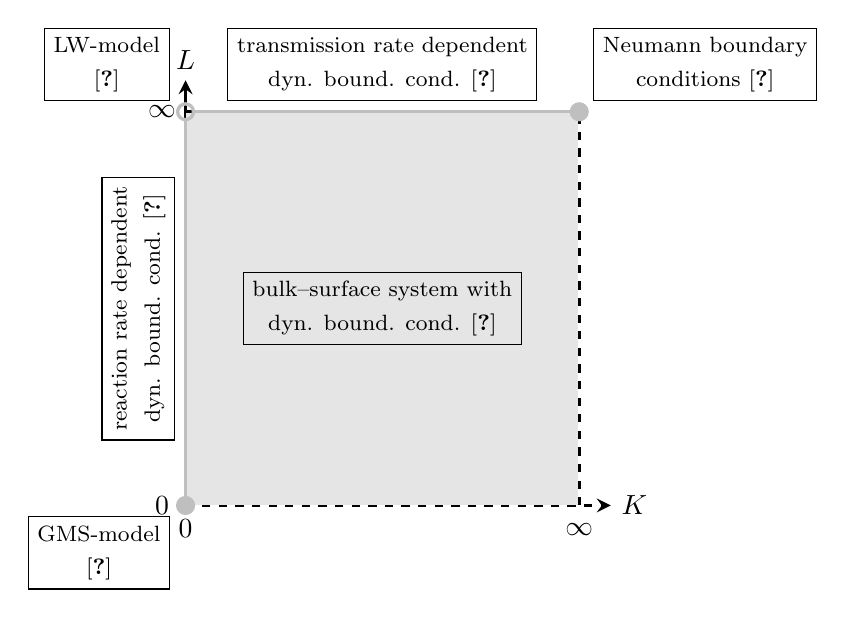
\begin{tikzpicture}
			\draw[-stealth, very thick, dashed] (0,0)  -- (5.4,0) node[right] {$K$}; 
			\node at (0,-0.3) {$0$};
			\node at (5,-0.3) {$\infty$};
			\draw[-stealth, very thick] (0,0)  -- (0,5.4) node[above] {$L$}; 
			\node at (-0.3,0) {$0$};
			\node at (-0.3,5) {$\infty$};
			
			\draw[dashed, very thick] (5,0) -- (5,5);
			\draw[dashed, very thick] (0,5) -- (5,5);
			
			\node[draw,align=center] at (-1,5.6) {\footnotesize LW-model \\ \footnotesize \cite{LiuWu2019}};
			
			\node[draw,align=center] at (2.5,5.6) {\footnotesize transmission rate dependent \\ \footnotesize dyn. bound. cond. \cite{KnopfLam2020}};
			
			\node[draw,align=center] at (-1.1,-0.6) {\footnotesize GMS-model \\ \footnotesize \cite{GoldsteinMiranvilleSchimperna2011}};
			
			\node[draw,rotate=90, align=center] at (-0.6,2.5) {\footnotesize reaction rate dependent \\ \footnotesize dyn. bound. cond. \cite{KnopfLamLiuMetzger2021}};
			
			\node[draw,align=center] at (6.6,5.6) {\footnotesize Neumann boundary \\ \footnotesize conditions \cite{CahnHilliard1958}};
			
			
			
			\fill[gray!20] (0.01,0.01) rectangle (4.99,4.99);
			
			\draw[gray!50, very thick] (0,5) circle (0.1);
			%	\draw[blue!50, very thick] (6,0) circle (0.1);
			\filldraw[color=gray!50, fill=gray!50, very thick] (0,0) circle (0.1);
			\filldraw[color=gray!50, fill=gray!50, very thick] (5,5) circle (0.1);
			
			\node[draw,align=center] at (2.5,2.5) {\footnotesize bulk--surface system with \\ \footnotesize dyn. bound. cond. \cite{KnopfStange2024}};
			
			\draw[gray!50, very thick] (0.1,5) -- (5,5);
			\draw[gray!50, very thick] (0,0.1) -- (0,4.9);
			%\draw[blue!50, very thick] (0.1,0) -- (5.9,0);
			
		\end{tikzpicture}
	\end{adjustbox}
	\caption{Sketch of the different types of dynamic boundary conditions corresponding to the parameter-choices $K,L \in [0,\infty]$. The main result of this paper, Theorem~\ref{thm:OptimalOrderErrorEst} shows optimal-order error estimates for the range of parameters marked in gray (the domain $[0,\infty]^2$ except circles and dashed lines).}\label{fig:graphDynBC}
\end{figure}

\section{Notation and Preliminaries}

\label{section:Notation}
\subsection*{Notation} We use the following notation throughout the paper: For $1 \leq p \leq \infty$ and $k\geq 0$ we denote the standard Lebesgue spaces on $\Om \subset \R^d$ by $L^p(\Om)$ and the Sobolev spaces by $W^{k,p}(\Om)$ (see, e.g., \cite[Section~5.2.2]{Evans1998}). For $p=2$ we use the standard notation for the Hilbert spaces $H^k(\Om)=W^{k,2}(\Om)$. For the Lebesgue and Sobolev spaces on $\Ga=\partial \Om$ we use the similar notation $L^p(\Ga)$ and $W^{k,p}(\Ga)$ (see, e.g., \cite[Definition 2.11]{DziukElliott2013}). For any Banach space $X$, we denote by $\| \cdot \|_X$ its norm, by $X'$ the dual space and the associated duality pairing by $\langle \cdot , \cdot \rangle_X$. For a Hilbert space $X$ we denote the inner product by $(\cdot , \cdot )_X$ and if $u \in L^1(\Om)$, respectively $u \in L^1(\Ga)$, we define the spatial mean on $\Om$, respectively $\Ga$, as
\begin{align*}
	\langle u \rangle_\Om := \frac{1}{|\Om|} \int_\Om u , \quad \text{respectively } \langle u \rangle_\Ga := \frac{1}{|\Ga|} \int_\Ga u .
\end{align*}

\subsection*{Preliminaries}
\begin{itemize}
	\item[(P1)] \label{eq:Preliminary1}Let $\nu$ denote the unit outward pointing normal vector to $\Ga$, then we define the surface gradient $\nabla_\Ga$ of a function $u:\Ga \to \mathbb{R}$ by $\nabla_\Ga u := \nabla \bar u - (\nabla \bar u \cdot \nu)\nu$, where $\bar u$ is an arbitrary extension of $u$ in a neighborhood of $\Ga$. The Laplace--Beltrami operator on $\Ga$ is given by $\Delta_\Ga u = \nabla_\Ga \cdot \nabla_\Ga u$. Moreover, $\gamma u$ denotes the trace of $u$ on $\Ga$, for brevity we will mostly suppress the trace operator in the notation below. The normal derivative of $u$ on $\Ga$ is denoted by $\partial_\nu u$. For a more explicit definition of these operators, see \cite[Section~2.2]{DziukElliott2013} and \cite[Section~5.5]{Evans1998}.
	
	%	\item[(P2)] \label{eq:Preliminary2} We define the Hilbert spaces
	%	\begin{align*}
		%		V := \{\phi \in H^1(\Om) : \phi|_{\Ga} \in H^1(\Ga)\} \subset H:=L^2(\Om) \times L^2(\Ga),
		%	\end{align*}
	%	with norms given by
	%	\begin{align*}
		%		\| u \|_V^2:=&\  \| u \|_{H^1(\Om)}^2 + \| u \|_{H^1(\Ga)}^2, \\
		%		\|(u_\Om,u_\Ga)\|_H^2:=&\  \| u_\Om \|_{L^2(\Om)}^2 + \| u_\Ga \|_{L^2(\Ga)}^2.
		%	\end{align*}
	%	Additionally we define the seminorm
	%	\begin{align*}
		%		|v|^2:=|v|_\Om^2 + |v|_\Ga^2 = \int_{\Om} |\nabla v|^2 + \int_{\Ga} |\nabla_\Ga v|^2 ,
		%	\end{align*}
	%	for $v \in V$. This is in line with the abstract setting introduced in \cite[Section~2.1.1]{KovacsLubich2017} for parabolic problems with dynamic boundary conditions. We have the Gelfand triple (see, e.g., \cite{Thomee2006}), with dense embeddings
	%	\begin{align*}
		%		V \hookrightarrow H\simeq H^\ast \hookrightarrow V^\ast ,
		%	\end{align*}
	%	in particular with the continuous and dense embedding $V \hookrightarrow H$ given by $v \mapsto (v,\gamma v)$. As a consequence, the duality pairing $\langle \cdot , \cdot \rangle_V\colon V^\ast \times V \to \mathbb{R}$ coincides with $m(\cdot
	%	
	%	We additionally define the weak dual norms, with the definitions in \hyperref[eq:Preliminary3]{(P2)}, for $d \in V$:
	%	\begin{equation*} 
		%		\begin{aligned},\cdot)$ on $H\times V$, defined in \hyperref[eq:Preliminary3]{(P2)}. For $u \in V$ we often abbreviate pairs $ (u,\gamma u) \in H$ by their first argument $u$. 
			%			\| d \|_{\ast,1}:= \sup_{0\not=\varphi \in V}\frac{m(d,\varphi)}{\|\varphi\|_V},\\
			%			\| d \|_{\ast,2}:= \sup_{0\not=\varphi \in V}\frac{m(d,\varphi)}{\|\varphi\|_{H^1(\Om)}},\\
			%			\| d \|_{\ast,3}:= \sup_{0\not=\varphi \in V}\frac{m_{\Ga}(d,\varphi)}{|\varphi|_{L^2(\Ga)}}.
			%		\end{aligned}
		%	\end{equation*}
	%	\NBon P2 has to be changed \NBoff
	
	\item[(P2)] \label{eq:Preliminary2} We introduce for a parameter $J\in [0,\infty]$ and $\lambda \in \R$ the combined Hilbert spaces
	\begin{align*}
		&H:= L^2(\Om) \times L^2(\Ga), \quad D^\lambda:=\{ (\phi,\psi) \in H^1(\Om) \times H^1(\Ga) \colon \phi=\lambda \psi \text{ a.e. on } \Ga \}, \\
		&\text{and }\qquad  V^{J,\lambda}:=\begin{cases}
			H^1(\Om) \times H^1(\Ga), \quad &\text{if } J\in (0,\infty] \\
			D^\lambda, \quad &\text{if } J=0
		\end{cases}.
	\end{align*}
	%	with the scalar products
	%	\begin{align*}
		%		(\cdot,\cdot)_H:=m(\cdot,\cdot):= (\cdot,\cdot)_{L^2(\Om)} + (\cdot,\cdot)_{L^2(\Ga)}, \qquad (\cdot,\cdot)_{V^{J,\lambda}}:= a^\ast(\cdot,\cdot):= (\cdot,\cdot)_{H^1(\Om)} + (\cdot,\cdot)_{H^1(\Ga)}.
		%	\end{align*}
	Following the notation from \cite[Section~2.1.1]{KovacsLubich2017}, we introduce the following bilinear forms
	\begin{equation*}
		\begin{aligned}
			m:=(\cdot,\cdot)_H \colon &H \times H \to \mathbb{R} ,\\
			& \big((\phi,\psi),(\zeta,\xi)\big) \mapsto  \int_\Om \phi  \zeta + \int_\Ga  \psi \xi  , \\
			a^\ast:=(\cdot,\cdot)_{V^{J,\lambda}} \colon &V^{J,\lambda} \times V^{J,\lambda} \to \mathbb{R} ,\\
			& \big((\phi,\psi),(\zeta,\xi)\big) \mapsto  \int_\Om \nabla \phi \cdot \nabla \zeta + \int_\Om \phi  \zeta + \int_\Ga \nabla_\Ga \psi \cdot \nabla_\Ga \xi + \int_\Ga  \psi \xi  , \\
			a^{J,\lambda} \colon &V^{J,\lambda} \times V^{J,\lambda} \to \mathbb{R} ,\\
			&\big((\phi,\psi),(\zeta,\xi)\big) \mapsto  \int_\Om \nabla \phi \cdot \nabla \zeta + \int_\Ga \nabla_\Ga \psi \cdot \nabla_\Ga \xi  + \h(J) \int_\Ga (\lambda \psi-\phi)(\lambda \xi-\zeta) ,  
		\end{aligned}
	\end{equation*}
	and the semi-norm
	\begin{align*}
					|\cdot|_{a^{J,\lambda}} \colon &V^{J,\lambda} \to \mathbb{R} ,\\
					& (\phi,\psi) \mapsto  \Big(a^{J,\lambda}((\phi,\psi),(\phi,\psi))\Big)^{\frac12},
	\end{align*}
	where we set 
	\begin{align*}
		\h(J):= \begin{cases}
			J^{-1}, \qquad &\text{if }J\in(0,\infty),\\
			0, \qquad &\text{if }J\in \{0,\infty\}
		\end{cases}.
	\end{align*}
	
	We additionally define the weak dual norms, for $d \in H$:
	\begin{equation} \label{eq:dualNormDef} 
		\begin{aligned}
			\| d \|_{\ast,J,\lambda}:= \sup_{0\not=\varphi \in V^{J,\lambda}}\frac{m(d,\varphi)}{\|\varphi\|_{V^{J,\lambda}}}.
		\end{aligned}
	\end{equation}
	\item[(P3)] \label{eq:Preliminary3} Since the choice of $m_\Om$, $m_\Ga$, $\epsilon, \delta$ and $\kappa$ has no impact on the mathematical analysis, we simply set, without loss of generality, $m_\Om=m_\Ga=\epsilon=\delta=\kappa=1$ for the remainder of the theoretical part of this paper. 
	
	Following \cite{KnopfStange2024}, a weak solution of the system \eqref{eq:CHreact} on $[0,T]$, for $K,L \in [0,\infty]$ and $(u_0,\psi_0) \in V^{K,\alpha}$, is a quadruplet $(u,\psi,\mu,\theta)$, satisfying the following properties:
	\begin{enumerate}
		\item[i)] The functions $u$, $\psi$, $\mu$ and $\theta$ have the regularity:
		\begin{equation} \label{eq:WeakFormReg}
			\begin{aligned}
				&(u,\psi) \in C([0,T];H) \cap H^1(0,T;(V^{L,\beta})') \cap L^\infty(0,T;V^{K,\alpha}), \\
				&(\mu,\theta) \in L^2(0,T;V^{L,\beta}). 
			\end{aligned} 
		\end{equation} 
		\item[ii)] The functions $u$ and $\psi$ satisfy the initial conditions $u|_{t=0}=u_0$ a.e. in $\Om$, and $\psi|_{t=0}=\psi_0$ a.e. on $\Ga$.
		\item[iii)] The functions $u$, $\psi$, $\mu$ and $\theta$ satisfy the weak formulation
		\begin{subequations} \label{eq:CHweak}
			\begin{align}
				m\big((\partial_t u, \partial_t \psi),(\zeta,\xi)\big) + a^{L,\beta}\big((\mu,\theta),(\zeta,\xi)\big) =&\ 0, \label{eq:CHweak1}\\
				m\big((\mu, \theta),(\eta,\vartheta)\big) - a^{K,\alpha}\big((u,\psi),(\eta,\vartheta)\big) =&\  m\big((F_\Om'(u),F_\Ga'(\psi)),(\eta,\vartheta)\big),\label{eq:CHweak2}
			\end{align}
		\end{subequations}
		a.e. in $[0,T]$, for all $(\zeta,\xi) \in V^{L,\beta}$, $(\eta,\vartheta) \in V^{K,\alpha}$.
		\item[iv)] The functions $u$ and $\psi$ satisfy the mass conservation law
		\begin{align} \label{eq:MassConservation}
			\begin{cases}
				\beta \int_\Om u(t) + \int_\Ga \psi(t) = \beta \int_\Om u_0 + \int_\Ga \psi_0, \qquad \text{if } L\in [0,\infty), \\
				\int_\Om u(t) = \int_\Om u_0 \text{ and } \int_\Ga \psi(t) = \int_\Ga \psi_0, \qquad \text{if } L=\infty,
			\end{cases}
		\end{align}
		for all $t\in [0,T]$. This can be obtained by testing \eqref{eq:CHweak1} with $(\beta,1) \in V^{L,\beta}$ and integrating over $t$.
		\item[v)] The functions $u$ and $\psi$ satisfy the energy inequality
		\begin{align*}
			E_K(u(t),\psi(t)) + \int_0^t \int_\Om |\nabla \mu|^2 + \int_0^t \int_\Ga |\nabla_\Ga \theta|^2 + \h(L) \int_0^t \int_\Ga |\beta\theta - \mu|^2 \leq E_K(u_0,\psi_0),
		\end{align*}
		for all $t \in [0,T]$ and the Ginzburg-Landau bulk--surface free energy
		\begin{align*}
			E_K(u,\psi):=&\ \int_\Om \frac\epsilon2 |\nabla u|^2 + \int_\Om \epsilon^{-1}F_\Om(u) + \int_\Ga \frac{\delta\kappa}{2} |\nabla_\Ga \psi|^2 + \int_\Ga \delta^{-1}F_\Ga(u) \nonumber \\
			&\ + \h(K) \int_\Ga \frac12 |\alpha \psi - u|^2.
		\end{align*}
		This can be obtained by testing \eqref{eq:CHweak1} with $(\mu,\theta) \in V^{L,\beta}$, subtracting \eqref{eq:CHweak2} tested with $(\partial_t u,\partial_t \psi) \in V^{K,\alpha}$ and integrating over $t$.
	\end{enumerate}
	
	The main result in \cite[Theorem 3.2]{KnopfStange2024} provides existence and high regularity of weak solutions, satisfying i)-v), for the bulk--surface Cahn--Hilliard system with dynamic boundary conditions \eqref{eq:CHreact}. This result requires polynomial growth conditions on the nonlinear potentials, which include, for example, the important double well potential. 
	\begin{rem}
		We will mostly work with this abstract formulation of the problem to showcase that the following arguments can be applied in a more general setting, we therefore expect that this strategy of proof can be adapted to a wider class of problems, see, e.g., Section~\ref{section:Generalization} for the optimal-order convergence result for the Cahn--Hilliard equation on an evolving surface.
	\end{rem}
\end{itemize}

\subsection*{Assumption}
\begin{itemize}
	\item[(A)] \label{eq:AssumptionPara} Let $\Om \subset \mathbb{R}^d$, for $d=2,3$, be a bounded domain with an (at least) $C^2$ boundary $\Ga=\partial \Om$.	We assume for the parameters
	\begin{itemize}
		\item $K\in [0,\infty)$, $L\in (0,\infty)$: $\alpha\beta|\Om| + |\Ga| \not= 0$, required for the bulk--surface Poincar\'e--Wirtinger inequality, cf. Lemma~\ref{Lemma:BulkSurfPoincare}.
		\item $K\in (0,\infty)$, $L=\infty$: $\alpha \not=0$ and a $C^3$-boundary $\Ga$.
		\item $K =  0$, $L=0$: $\alpha\beta|\Om| + |\Ga| \not= 0$ and $F_\Om'(\alpha \cdot)=\beta F_\Ga'(\cdot)$ for the nonlinear potentials.
	\end{itemize}
\end{itemize}





\section{Full discretization of the bulk--surface Cahn--Hilliard system with dynamic boundary conditions}
\label{section:Discretization CH}

\subsection{Bulk--surface finite elements} \label{sec:bulk--surfaceFEM}
In order to discretize the equation in space, we use the linear finite element method for partial differential equations developed by Elliott and Ranner \cite[Sections 4,5]{ElliottRanner2013} and by \cite[Section~4]{KovacsLubich2017}, see also \cite[Sections 4-7]{ElliottRanner2021}. 

We approximate the domain $\Om$ by a polyhedral domain $\Om_h$ and take a quasi-uniform triangulation $\calT_h$ of $\Om_h$ (see \cite[Definition 4.4.13]{BrennerScott2008}). This triangulation consists of closed simplices, either triangles in $\mathbb{R}^2$ or tetrahedra in $\mathbb{R}^3$. Let $\Ga_h:=\partial \Om_h$, then the faces of $\Ga_h$ are $(d-1)$-simplices, hence edges in $\mathbb{R}^2$ or triangles in $\mathbb{R}^3$, and we assume that the vertices lie on $\Ga$. We define the mesh width as $h=\max\{\text{diam}(T) \colon T \in \calT_h\}$ and assume that the mesh width is sufficiently small, such that for all $x \in \Ga_h$, there exists a unique point $p(x) \in \Ga$, such that $x-p(x)$ is orthogonal to the tangent space of $\Ga$ at $p$, for more details on the construction see \cite[Section~4]{ElliottRanner2013}.

We define the non-conforming finite element space $V_h\nsubseteq H^1(\Om)$, corresponding to $\calT_h$, by the continuous, piecewise linear nodal basis functions on $\Om_h$: Let $(x_k)_{k=1}^N$ be the collection of all nodes of the triangulation in $\Om_h$, then we define $(\phi_j)_{j=1}^N$ as the family of continuous functions, which are piecewise linear on each of the simplices of $\calT_h$, subject to the condition
\begin{align*}
	\phi_j(x_k)=\delta_{jk} \text{ for } j,k=1,...,N. 
\end{align*}
Then the \emph{bulk} finite element space is defined as $V_h:= \Span\{\phi_1,...,\phi_N\}$.

If we use, without loss of generality, that the nodes of the triangulation $\calT_h$ on the boundary $\Ga_h$ are the nodes $(x_k)_{k=1}^M$, then the \emph{surface} finite element space $S_h\nsubseteq H^1(\Ga)$ is given by
\begin{align*}
	S_h:=  \Span\{\phi_1|_{\Ga_h},...,\phi_M|_{\Ga_h}\}.
\end{align*}
These definitions are carried out in more detail in \cite[Section~6.2]{ElliottRanner2021}.

Next we define the lift operator $\cdot^\ell \colon V_h \to V_h^\ell$ of functions $v_h \colon \Om_h \to \mathbb{R}$ to $v_h^\ell \colon \Om \to \mathbb{R}$ by setting $v_h^\ell(p)=v_h(x)$ for $x\in \Om_h$ and $p \in \Om$, which are related as described in detail in \cite[Section~4]{ElliottRanner2013}, and by defining
\begin{align*}
	V_h^\ell:=\{v_h^\ell : v_h \in V_h\}.
\end{align*}
For functions $v_h \in S_h$ on the discrete surface this lift operator is then given by
\begin{align*}
	v_h^\ell \colon \Ga \to \mathbb{R} \qquad \text{with } v_h^\ell(p)=v_h(x) ,\quad \forall p\in \Ga,
\end{align*}
where $x \in \Ga_h$ is the unique point on $\Ga_h$ with $x-p$ orthogonal to the tangent space $T_p\Ga$.

The discrete gradient $\nabla_h$ and tangential gradient $\nabla_{\Ga_h}$ are piecewisely defined analogously to $\nabla$ and $\nabla_\Ga$, see \cite[Section~4]{DziukElliott2013}. The discrete trace operator $\gamma_h v_h$ is defined by the restriction of the continuous functions $v_h \in V_h$ onto $\Ga_h$, with the same notational conventions as before, e.g. $\nabla_{\Ga_h}v_h:=\nabla_{\Ga_h}(\gamma_h v_h)$.

For the combined bulk--surface system we define analogous to the analytic spaces in \hyperref[eq:Preliminary2]{(P2)} the \emph{bulk--surface} finite element space, for $J\in [0,\infty]$ and $\lambda \in \R$ as
\begin{align}
	V_{h}^{J,\lambda}:=\begin{cases}
		V_h \times S_h, \qquad &\text{if } J\in (0,\infty],\\
		D_{h}^{\lambda}:=\{(v_h,s_h) \in V_h \times S_h \colon v_h|_{\Ga_h}=\lambda s_h\}, \qquad &\text{if } J=0.
	\end{cases}\label{eq:DefFESpace}
\end{align}


\subsection{Linearly implicit backward difference time discretization\protect\footnote{Up to some changes, the text of this preparatory subsection is taken from \cite[Section~4]{BullerjahnKovacs2024}.}} \label{sec:BDF}
We combine the discretization in space by the bulk--surface finite elements with the following discretizations in time: Let $q=1,\dotsc,5$, $\tau >0$ be the time step size, and $q\tau \leq t_n:=n\tau \leq T$ be a uniform partition of the time interval $[0,T]$. We assume the starting values $(u_h^0,\psi_h^0), \dots, (u_h^{q-1},\psi_h^0) \in V_h^{K,\alpha}$ to be given, and define, for $q\leq n$, the discretized time derivative, and the extrapolation for the non-linear term, respectively, as
\begin{equation*}\label{eq:DefdiscDerivandExtra}
	\begin{aligned}
		&\partial^\tau_q u_h^n:= \frac{1}{\tau} \sum_{j=0}^q \delta_j u_h^{n-j},\qquad	&&\widetilde u_h^n:= \sum_{j=0}^{q-1} \gamma_j u_h^{n-1-j}, \\
		&\partial^\tau_q \psi_h^n:= \frac{1}{\tau} \sum_{j=0}^q \delta_j \psi_h^{n-j},\qquad	&&\widetilde \psi_h^n:= \sum_{j=0}^{q-1} \gamma_j \psi_h^{n-1-j}.
	\end{aligned}
\end{equation*}
Where the coefficients are given by the expressions
\begin{subequations}\label{eq:BdfCoeff}
	\begin{align}
		\label{eq:BDF generating function}
		\delta(\zeta)=&\sum_{j=0}^q \delta_j \zeta^j=\sum_{l=1}^q \frac{1}{l} (1-\zeta)^l, \\
		\gamma(\zeta)=&\sum_{j=0}^{q-1}\gamma_j \zeta^j=\frac{(1-(1-\zeta)^q)}{\zeta}.
	\end{align}
\end{subequations}

The $q$-step BDF methods are of order $q$, they are $A$-stable for $q=1,2$, $A(\alpha_q)$-stable for $q=3,\dotsc,6$ with $\alpha_3 =86.03^\circ$, $\alpha_4=73.35^\circ$, $\alpha_5=51.84^\circ$,  and $\alpha_6 = 17.84^\circ$, respectively, and unstable for $q \geq 7$, see, e.g.,  \cite[Section~V.2]{HairerWanner1996}, \cite[Section~2.3]{AkrivisLubich2015}, while see \cite{AkrivisKatsoprinakis2020} for the exact $\alpha_q$ values. 

The starting values can be precomputed using either a lower order method with smaller time step size, or a Runge--Kutta method of suitable order.

\subsection{The fully discrete scheme in abstract form}

We apply the bulk--surface finite element approximation (see subsection \ref{sec:bulk--surfaceFEM}) to the abstract variational formulation \eqref{eq:CHweak} of the bulk--surface Cahn--Hilliard system with dynamic boundary conditions, namely we discretize the integrals in the bilinear forms, defined in \hyperref[eq:Preliminary2]{(P2)} for $J\in[0,\infty]$ and $\lambda \in \R$, by integrals over the polyhedral domains $\Om_h$ and $\Ga_h$, following \cite[Section~4.1]{KovacsLubich2017}, for the space $V_h^{J,\lambda}$ defined in \eqref{eq:DefFESpace}:
\begin{equation*} \label{eq:DefDiscBilinearForms}
	\begin{aligned}
		m_h \colon &V_h^{J,\lambda} \times V_h^{J,\lambda} \to \mathbb{R} ,\\
		 &\big((\phi_h,\psi_h),(\zeta_h,\xi_h)\big) \mapsto  \int_{\Om_h} \phi_h \zeta_h + \int_{\Ga_h} \psi_h \xi_h ,\\
		%&m_{\Ga_h} \colon S_h \times S_h \to \mathbb{R} ,\qquad &&(\phi_h,\psi_h) \mapsto  \int_{\Ga_h} \phi_h \psi_h , \\
		a_h^{\ast} \colon &(V_h\times S_h) \times (V_h \times S_h) \to \mathbb{R} ,\\
		&\big((\phi_h,\psi_h),(\zeta_h,\xi_h)\big) \mapsto  \int_{\Om_h} \nabla_h \phi_h \cdot \nabla_h \zeta_h + \int_{\Om_h} \phi_h \zeta_h +  \int_{\Ga_h} \nabla_{\Ga_h} \psi_h \cdot \nabla_{\Ga_h} \xi_h + \int_{\Ga_h} \psi_h \xi_h  , \\	
		a_h^{J,\lambda} \colon &V_h^{J,\lambda} \times V_h^{J,\lambda} \to \mathbb{R} ,\\
		&\big((\phi_h,\psi_h),(\zeta_h,\xi_h)\big) \mapsto \int_{\Om_h} \nabla_h \phi_h \cdot \nabla_h \zeta_h + \int_{\Ga_h} \nabla_{\Ga_h} \psi_h \cdot \nabla_{\Ga_h} \xi_h  \nonumber \\
		&\hphantom{\big((\phi_h,\psi_h),(\zeta_h,\xi_h)\big) \mapsto} + \h(J) \int_{\Ga_h} (\lambda \psi_h - \phi_h) (\lambda \xi_h-\zeta_h) .	 
	\end{aligned}
\end{equation*}
Note that we define the discrete norms and the semi-norm analogous to the continuous case by
\begin{align}
	\| \cdot \|_{H_h}^2:=m_h(\cdot,\cdot), \quad \| \cdot \|_{V_h^{J,\lambda}}^2:=a_h^\ast(\cdot,\cdot), \quad |\cdot |_{a_h^{J,\lambda}}^2:=a_h^{J,\lambda}(\cdot,\cdot). \label{eq:DefDiscNorms}
\end{align}

Then we use a Galerkin ansatz in order to solve this variational problem in a finite element space and combine this with the discretization in time by the $q$-step linearly implicit backwards difference method (see Section \ref{sec:BDF}). Then the fully discrete scheme reads: Let $L,K \in [0,\infty]$, then find, for $h,\tau >0$ and $q \tau \leq t_n:=n\tau \leq T$, functions $(u_h^n, \psi_h^n) \in V_h^{K,\alpha}$ and $(\mu_h^n,\theta_h^n) \in V_h^{L,\beta}$ such that
\begin{subequations} \label{eq:CHweakD}
	\begin{align}
		m_h\big((\partial_q^\tau u_h^n, \partial_q^\tau \psi_h^n),(\zeta_h,\xi_h)\big) + a_h^{L,\beta}\big((\mu_h^n,\theta_h^n),(\zeta_h,\xi_h)\big) =&\ 0, \label{eq:CHweakD1}\\
		m_h\big((\mu_h^n, \theta_h^n),(\eta_h,\vartheta_h)\big) - a_h^{K,\alpha}\big((u_h^n,\psi_h^n),(\eta_h,\vartheta_h)\big) =&\  m_h\big((F_\Om'(\widetilde u_h^n),F_\Ga'(\widetilde\psi_h^n)),(\eta_h,\vartheta_h)\big).\label{eq:CHweakD2}
	\end{align}
\end{subequations}
for all $(\zeta_h,\xi_h) \in V_h^{L,\beta}$ and $(\eta_h,\vartheta_h) \in V_h^{K,\alpha}$ and with initial values $(u_h^0,\psi_h^0),...,(u_h^{q-1},\psi_h^{q-1}) \in V_h^{K,\alpha}$ given. 


\section{Main result: Optimal-order fully discrete error estimates}
\label{section:MainResult}
The main result of this paper establishes optimal-order error estimates for the bulk--surface finite element and linearly implicit backward difference discretization of the bulk--surface Cahn--Hilliard system with dynamic boundary conditions \eqref{eq:CHweak}, for the range of parameters depicted in Figure~\ref{fig:graphDynBC}, cf. \hyperref[eq:AssumptionPara]{(A)}. For the GMS-model, i.e. the choice $K=0$ and $L=0$, this result was already obtained in \cite{BullerjahnKovacs2024}, by a different technique of exploiting the anti-symmetric structure of the equation, which is not possible in the general case. To our knowledge there are no fully discrete error estimates available for other choices of parameters $K$ and $L$, note however that convergence of sub-sequences without rates are available.

\begin{thm}\label{thm:OptimalOrderErrorEst}
	Let $1\leq q \leq 5$ and $(u,\psi,\mu,\theta)$ be a sufficiently smooth solution (see \eqref{eq:regularityAss}) of the bulk--surface Cahn--Hilliard system with dynamic boundary conditions \eqref{eq:CHweak}, with \hyperref[eq:AssumptionPara]{(A)} and nonlinear potentials satisfying \eqref{eq:RegAssPot}. Then there exists $h_0>0$ such that for all $h\leq h_0$ and $\tau >0$, satisfying the mild step size restriction $\tau^q\leq C_0 h^2$ (where $C_0$ can be chosen arbitrarily), the error between the solution $(u,\psi,\mu,\theta)$ and the fully discrete solution $(u_h^n,\psi_h^n,\mu_h^n,\theta_h^n)$ of \eqref{eq:CHweakD}, using linear bulk--surface finite element discretization and linearly implicit backward difference time discretization of order $q=1,\dots,5$, satisfies the optimal-order error estimates, for $q\tau \leq t_n:=n\tau \leq T$,
	\begin{align*}
		\| &(u^n_h)^\ell - u(t_n) \|_{L^2(\Om)} + \| (\psi^n_h)^\ell - \psi(t_n) \|_{L^2(\Ga)} \nonumber \\
		&+ h \Big( \| (u^n_h)^\ell - u(t_n) \|_{H^1(\Om)} + \|  (\psi^n_h)^\ell - \psi(t_n) \|_{H^1(\Ga)}\Big) \leq C (h^2+\tau^q),  \\
		\bigg( \tau \sum_{k=q}^n& \| (\mu^k_h)^\ell - \mu(t_k) \|_{L^2(\Om)}^2 + \|(\theta^k_h)^\ell - \theta(t_k) \|_{L^2(\Ga)}^2 \nonumber \\
		&+ h \Big(\| (\mu^k_h)^\ell - \mu(t_k) \|_{H^1(\Om)}^2 + \| (\theta^k_h)^\ell - \theta(t_k) \|_{H^1(\Ga)}^2\Big) \bigg)^{\frac{1}{2}} \leq C (h^2+\tau^q),
	\end{align*} 
	provided the error in the starting values $I_h^{q-1}$, defined in \eqref{eq:DefIhq}, is $O((\tau^q+h^2)^2)$. The constant $C>0$ depends on the Sobolev norms of the exact solution and exponentially on the final time $T$, but is independent of $h$ and $\tau$.
\end{thm}

\begin{rem}
	(i) The $h_0$ depends on geometric approximation results (see, e.g., Section~\ref{sec:bulk--surfaceFEM} and Section~\ref{section:Consistency}). The requirement on the smallness of both parameters is merely technical. 
	
	(ii) The mild step size restriction is needed to establish an $L^\infty$-bound on the error in the stability analysis. This lets us reduce the assumptions on the nonlinear potentials $F_\Om$ and $F_\Ga$ to a \emph{local} Lipschitz condition, which covers important examples such as the double well potential. The restriction can be even weakened to $\tau^q \leq C_0 h^{3/2+\epsilon_0}$, where $\epsilon_0,C_0 > 0$ can be chosen arbitrarily, as is apparent from the assumptions in Proposition~\ref{prop:stability}.
	
	(iii) The constant $C$ also depends on a polynomial expression of the inverses of $\epsilon$ and $\delta$, that is, limit processes for the interface parameters are not covered by our error estimates.
\end{rem}

Sufficient regularity assumptions for Theorem~\ref{thm:OptimalOrderErrorEst} are: The nonlinear potentials and their derivatives
\begin{equation}
	F_\Om^{(k)} \text{ and } F_\Ga^{(k)} \text{ are locally Lipschitz continuous for }k=0,\dots,3, \label{eq:RegAssPot}
\end{equation}
and the exact solutions satisfy the required regularity for the weak formulation \eqref{eq:WeakFormReg} and additionally
\begin{equation} \label{eq:regularityAss}
	\begin{alignedat}{3}
		&\ u \in H^{q+2}([0,T];H^2(\Om)), & \quad &
		\psi \in H^{q+2}([0,T];H^2(\Ga)), \\
		&\ \mu \in H^{3}([0,T];H^2(\Om)), & \quad &
		\theta \in H^{3}([0,T];H^2(\Ga)).
	\end{alignedat}
\end{equation}
Recall that by standard theory we have, for any $u \in H^1([0,T];X)$, that $u \in C([0,T],X)$ with
\begin{align*} 
	\max_{0\leq t \leq T} \| u(t)\|_X \leq c(T) \|u\|_{H^1([0,T];X)},
\end{align*}
see, e.g., \cite[Section~5.9.2]{Evans1998}. Since the Sobolev embedding $H^2 \subset L^\infty$ is continuous, by $d=2,3$ (see, e.g., \cite[Section~5.6.3]{Evans1998}), we have the regularity
\begin{equation*}
	\begin{aligned}
		u &\in W^{q+1,\infty}([0,T];L^{\infty}(\Om)), \quad && \psi \in  W^{q+1,\infty}([0,T];L^{\infty}(\Ga)), \\
		\text{and} \qquad \mu &\in W^{2,\infty}([0,T];L^\infty(\Om)), \quad &&~~\theta \in  W^{2,\infty}([0,T];L^\infty(\Ga)).
	\end{aligned}
\end{equation*}


\refstepcounter{scheme}
\begin{figure}[ht]	
	\renewcommand{\figurename}{Scheme} 
	\begin{itemize} 
		\item[\textbf{Part A}:] Derive an energy equality by testing the error equations with the errors and the discrete derivative of the errors
		
		\item[\textbf{Part $\text{B}_{\text{cont}}$}:](continuous case) Use the product rule and integration over $t$ to get the $H^1$-seminorm of the error at time $t$ on the left-hand side of the inequality
		
		\item[\textbf{Part $\text{B}_{\text{disc}}$}:] (fully discrete case) Use the technique based on the $G$-stability theory by Dahlquist \cite[Theorem~3.3]{Dahlquist1978} and the multiplier techniques of Nevanlinna and Odeh \cite[Section~2]{NevanlinnaOdeh1981}, sum over all time-steps and get the $H^1$-seminorm, of the error at time $t$ on the left-hand side of the inequality
		
		\item[\textbf{Part C}:] Eliminate terms in the (discrete) derivative of errors by a (discrete) product rule and re-substituting the equation, and then estimating the remaining terms
		
		\item[\textbf{Part D}:] Derive a Poincar\'e-type estimate by an \emph{almost mass conservation} of the error, to estimate the $H^1$-seminorm by the full $H^1$-norm 
		
		\item[\textbf{Part E}:] An absorption argument and Gr\"onwall's inequality yields the final estimate
	\end{itemize}
	\caption{General scheme of the new stability proof.}
	\label{scheme:Stability-scheme}
\end{figure}


In the following we will prove Theorem~\ref{thm:OptimalOrderErrorEst} by a combination of a stability and consistency analysis.

Scheme~\ref{scheme:Stability-scheme} captures the main new idea for the stability proof in this paper. Comparing this approach to the stability proof for the Cahn--Hilliard equation with Cahn--Hilliard type dynamic boundary conditions in \cite[Section~6]{BullerjahnKovacs2024}, this replaces a set of energy estimates, which depend heavily on the anti-symmetric structure of the equation, by only one energy estimate, and showing a discrete Poincar\'e-type inequality via an \emph{almost mass conservation} and the bulk--surface Poincar\'e-Wirtinger inequality, Lemma~\ref{Lemma:BulkSurfPoincare}. 

We therefore strongly believe that the stability Scheme~\ref{scheme:Stability-scheme} translates well to other equations satisfying an energy law and a mass conservation, allowing for similar stability results in a large class of problems, see, e.g., Section~\ref{section:Generalization} for the optimal-order convergence result for the Cahn--Hilliard equation on an evolving surface. 

To our knowledge this is the first time a fully discrete Poincar\'e-type inequality was used to show stability and convergence estimates for a higher order BDF time discretization. 

The transfer of the energy estimates from the continuous case to the fully discrete case is done by a method combining the $G$-stability theory by Dahlquist \cite[Theorem~3.3]{Dahlquist1978} and the multiplier techniques of Nevanlinna and Odeh \cite[Section~2]{NevanlinnaOdeh1981}, which has already proved to be effective for different partial differential equations, see, e.g., \cite{LubichMansourVenkataraman2013,AkrivisLubich2015,KovacsLiLubich2019,LLG,ContriKovacsMassing2023,HMHF,BullerjahnKovacs2024}.


In the consistency part we are concerned with the approximation error which comes from discretizations, and enters in the stability analysis as defect terms. The optimal-order fully discrete consistency bounds are obtained analogously to \cite[Section~7]{BullerjahnKovacs2024}, by error estimates for the spatial discretization, see, e.g. \cite[Section~6]{HarderKovacs2022}, and a sufficiently regular extension of the extrapolation to obtain error estimates for the backward difference time discretization.

A crucial advantage is that no shift by initial data is needed in the error analysis for the fully discrete scheme \eqref{eq:CHweakD} in comparison to the error analysis in \cite{KovacsLiLubich2021,HarderKovacs2022,BeschleKovacs2022,BullerjahnKovacs2024}.


\section{Bulk--surface Poincar\'e--Wirtinger inequality}

The key technical estimate in our stability proof is the Poincar\'e--Wirtinger inequality for the combined bulk and surface spaces introduced in \hyperref[eq:Preliminary2]{(P2)}. This result is the standard reformulation of the Poincar\'e-type estimate -- somewhat hidden -- in the appendix of \cite[Lemma~A.1]{KnopfLiu2021}, an earlier version for $J=0$ can be found in the appendix in \cite[Lemma~A]{ColliFukao2015}.

We define the generalized mean for bulk and surface functions, for $\lambda,\upsilon \in \R$, as
\begin{align*}
	M^{\lambda,\upsilon}\colon V^{J,\lambda} \to \R, \qquad (\phi,\psi) \mapsto \frac{\upsilon |\Om| \langle \phi \rangle_\Om + |\Ga| \langle \psi \rangle_\Ga}{\lambda \upsilon |\Om| + |\Ga|} ,
\end{align*}
and obtain the following result.
\begin{lem}[\bf Poincar\'e--Wirtinger inequality for bulk and surface] \label{Lemma:BulkSurfPoincare}
	Let $J\in [0,\infty)$ and $\lambda,\upsilon \in \R$, with $\lambda \upsilon |\Om| + |\Ga| \not=0$, and let $\Om \subset \R^d$ be a bounded Lipschitz domain with boundary $\Ga=\partial \Om$. Then there exists a constant $c_P >0$ depending only on $K$, $\lambda$, $\upsilon$ and $\Om$ such that 
	\begin{align*} 
		\Big\|\Big(\phi-\lambda M^{\lambda,\upsilon}((\phi,\psi)),\psi-M^{\lambda,\upsilon}((\phi,\psi))\Big)\Big\|_{V^{J,\lambda}} \leq c_P |(\phi,\psi)|_{a^{J,\lambda}}
	\end{align*}
	for all $(\phi,\psi) \in V^{J,\lambda}$.
\end{lem}
\begin{proof}
		The original proof in \cite[Lemma~A.1]{KnopfLiu2021} suffices here up to the mean zero transformations.
\end{proof}
In particular, this means that we obtain a Poincar\'e--Wirtinger inequality for the \emph{combined} bulk and surface, with the same combined mass $M^{\lambda,\upsilon}((\phi,\psi))$ in the bulk and on the surface. 

Note that if one would simply use the Poincar\'e-inequality in the bulk and on the surface \emph{independently}, one would need to use different masses for the bulk and surface part. This is not feasible since this problem in general only satisfies a conservation of the \emph{combined mass}, see \eqref{eq:MassConservation}.


\section{A continuous perturbation result} 
\label{section:ContPertProblem}

In order to familiarize and illustrate the main new idea of the stability proof in this paper, we first derive a continuous perturbation result, in the arguably simpler abstract setting, using Scheme~\ref{scheme:Stability-scheme}. In the stability analysis in Section~\ref{section:Stability} we will perform the same energy estimate transferred to the fully discrete case.

We start with a smooth solution $(u,\psi,\mu,\theta)$ of the bulk--surface Cahn--Hilliard system with dynamic boundary conditions \eqref{eq:CHweak}, with $K \in [0,\infty)$ and $L \in (0,\infty)$, and a smooth solution $(u^\ast, \psi^\ast, \mu^\ast, \theta^\ast)$ of a perturbed problem, where both equations in \eqref{eq:CHweak} are perturbed by smooth functions $(d^1,d^2,d^3,d^4)$. Within this section we additionally assume that $F_\Om'$ and $F_\Ga'$ are Lipschitz continuous, for simplicity. 

We are then interested in the errors $(e_u=u-u^\ast,e_\psi=\psi-\psi^\ast,e_\mu=\mu-\mu^\ast,e_\theta=\theta-\theta^\ast)$ which satisfy the error equations:
\begin{subequations} \label{eq:contError}
	\begin{align}
		m\big((\partial_t e_u, \partial_t e_\psi),(\zeta,\xi)\big) + a^{L,\beta}\big((e_\mu,e_\theta),(\zeta,\xi)\big) =&\ m\big((d_1,d_2),(\zeta,\xi)\big), \label{eq:contError1}\\
		m\big((e_\mu, e_\theta),(\eta,\vartheta)\big) - a^{K,\alpha}\big((e_u,e_\psi),(\eta,\vartheta)\big) =&\  m\big((r_\Om,r_\Ga),(\eta,\vartheta)\big) + m\big((d_3,d_4),(\eta,\vartheta)\big),\label{eq:contError2}
	\end{align}
\end{subequations}
for a.e. $t \in [0,T]$, for all $(\zeta,\xi) \in V^{L,\beta}$, $(\eta,\vartheta) \in V^{K,\alpha}$, and with the notation $r_\Om=F_\Om'(u)-F_\Om'(u^\ast)$ and $r_\Ga=F_\Ga'(\psi)-F_\Ga'(\psi^\ast)$.

Now we use Scheme~\ref{scheme:Stability-scheme} to prove a continuous perturbation estimate: 

\textbf{Part A}: We test \eqref{eq:contError1} with $(e_\mu,e_\theta)$ and subtract \eqref{eq:contError2} tested with $(\partial_t e_u,\partial_t e_\psi)$. This eliminates the mixed terms on the left-hand side of the equation and we have:
\begin{align*}
	&\ a^{K,\alpha}\big((\partial_t e_u,\partial_t e_\psi) , (e_u,e_\psi)\big) + | (e_\mu,e_\theta) |_{a^{L,\beta}}^2  \\
	&\ = -m\big((r_\Om,r_\Ga),(\partial_t e_u,\partial_t e_\psi)\big) - m\big((d^3,d^4),(\partial_t e_u,\partial_t e_\psi)\big)+ m\big((d^1,d^2),(e_\mu,e_\theta)\big).
\end{align*}

\textbf{Part $\text{B}_{\text{cont}}$}: We use the product rule and integration over $t \in (0,T]$ to arrive at
\begin{align*}
	&\frac{1}{2} | (e_u(t), e_\psi(t)) |_{a^{K,\alpha}}^2 + \int_0^t | ( e_\mu,e_\theta) |_{a^{L,\beta}}^2 \d s \\
	&\ = \frac{1}{2} | ( e_u(0), e_\psi(0)) |_{a^{K,\alpha}}^2 - \int_0^t m\big((r_\Om,r_\Ga),(\partial_t e_u,\partial_t e_\psi)\big)\d s  \\
	&\ - \int_0^t m\big((d^3,d^4),(\partial_t e_u,\partial_t e_\psi)\big)\d s+ \int_0^t m\big((d^1,d^2),(e_\mu,e_\theta)\big)\d s.
\end{align*}

\textbf{Part C}: We eliminate terms on the right-hand side involving the derivative of $e_u$ and $e_\psi$, by using \eqref{eq:contError1} and $L\not= 0$ to rewrite the terms involving the nonlinear potentials $F_\Om',F_\Ga'$, and using a product rule to rewrite the perturbation terms:
\begin{align*}
	- \int_0^t m\big((r_\Om,r_\Ga),(\partial_t e_u,\partial_t e_\psi)\big)\d s =&\ \int_0^t a^{L,\beta}\big((e_\mu,e_\theta),(r_\Om,r_\Ga)\big)\d s \nonumber \\
	&\ - \int_0^t m\big((d^1,d^2),(r_\Om,r_\Ga)\big)\d s, \\
	- \int_0^t m\big((d^3,d^4),(\partial_t e_u,\partial_t e_\psi)\big)\d s =&\ \int_0^t m\big((\partial_t d^3,\partial_t d^4),(e_u,e_\psi)\big)\d s \nonumber \\
	&\ - \int_0^t \frac{\d}{\d t} m\big((d^3,d^4),(e_u,e_\psi)\big)\d s.
\end{align*}
%\begin{align*}
%	&\ - \int_0^t \int_\Om r_\Om \partial_t e_u - \int_0^t \int_\Ga r_\Ga \partial_t e_\psi - \int_0^t \int_\Om d^3 \partial_t e_u  - \int_0^t\int_\Ga d^4 \partial_t e_\psi = \int_0^t \int_\Om \nabla e_\mu \nabla r_\Om + \int_0^t \int_\Ga \nabla_{\Ga} e_\theta \nabla_{\Ga}r_\Ga \\
%	&\ + \h(L) \int_\Ga (\beta e_\theta - e_\mu)(\beta r_\Ga - r_\Om) - \int_0^t \int_\Om d^1 r_\Om - \int_0^t \int_\Ga d^2 r_\Ga \\
%	&\ - \int_0^t \frac{\d}{\d t}\int_\Om d^3 e_u + \int_0^t \int_\Om \partial_t d^3 e_u  - \int_0^t \frac{\d}{\d t} \int_\Ga d^4 e_\psi  + \int_0^t \int_\Ga \partial_t d^4 e_\psi\\
%\end{align*}

For the perturbations we use the dual norm defined in \eqref{eq:dualNormDef}, Cauchy--Schwarz and Young's inequalities, and we use Lipschitz continuity to estimate the nonlinear terms $r_\Om$ and $r_\Ga$ by $e_u$ and $e_\psi$, to arrive at the estimate
\begin{align}
	\frac{1}{2} | (e_u(t), e_\psi(t)) |_{a^{K,\alpha}}^2 + \int_0^t | ( e_\mu,e_\theta) |_{a^{L,\beta}}^2\d s \leq&\  \delta \| (e_u(t),e_\psi(t)) \|_{V^{K,\alpha}}^2 +\delta \int_0^t\| (e_\mu,e_\theta) \|_{V^{L,\beta}}^2\d s \nonumber \\
	&\ + c \int_0^t \| (e_u,e_\psi) \|_{V^{K,\alpha}}^2\d s + c(D +I), \label{eq:contErrorest1}
\end{align}
%	\begin{align*}
	%		\frac{\d}{\d t} \Big( \frac{1}{2} \| \nabla e_u \|_H^2 \Big) + \| \nabla e_\mu \|_{L^2(\Om)}^2 + \| \nabla_\Ga e_\theta \|_{L^2(\Ga)}^2 + \frac{1}{L} \| e_\theta - e_\mu \|_{L^2(\Ga)}^2 \leq&\ \delta \| e_\mu \|_{H^1(\Om)}^2 +\delta \| \nabla_\Ga e_\theta \|_{L^2(\Ga)}^2 +\delta \|e_\theta - e_\mu \|_{L^2(\Ga)}^2 \\
	%		&\ + c \| e_u \|_V^2 - \frac{\d}{\d t} \Big( \int_\Om d^2 e_u  + \int_\Ga d^2 e_u \Big) + cD 
	%	\end{align*}
where $\delta>0$ is the constant from Young's inequality and can be chosen arbitrarily small to absorb terms into the left-hand side. We collect the initial errors in $I:= | ( e_u(0), e_\psi(0)) |_{a^{K,\alpha}}^2$ and the terms coming from the perturbation into:
\begin{align*}
	D:=&\ \| (d^3(t),d^4(t)) \|_{\ast,K,\alpha}^2 + \| (d^3(0),d^4(0)) \|_{\ast,K,\alpha}^2 + \int_0^t \| (d^1,d^2) \|_{\ast,L,\beta}^2\d s \nonumber \\
	&\ + \int_0^t \| (d^3,d^4) \|_{\ast,K,\alpha}^2\d s + \int_0^t \| (\partial_t d^3,\partial_t d^4) \|_{\ast,K,\alpha}^2\d s .
\end{align*}

%	\begin{align}
	%		\| \nabla e_u \|_H^2 + + \int_0^t \| \nabla e_\mu \|_{L^2(\Om)}^2 + \int_0^t\| \nabla_\Ga e_\theta \|_{L^2(\Ga)}^2 + \frac{1}{L} \int_0^t \| e_\theta - e_\mu \|_{L^2(\Ga)}^2 \leq&\ \delta \int_0^t \| e_\mu \|_{H^1(\Om)}^2 + c \int_0^t \| e_u \|_V^2 \nonumber \\
	%		&\ + \delta \| e_u \|_V^2 + c(D +I ).\label{eq:contErrorest1}
	%	\end{align}

\textbf{Part D}: We would like to derive a Poincar\'e-type inequality, but unfortunately the functions $e_u$, $e_\psi$, $e_\mu$, and $e_\theta$ do not satisfy a mass conservation. But we obtain, by testing \eqref{eq:contError1} with the constant functions $(\beta,1)\in V^{L,\beta}$, the 
\begin{equation} \label{eq:AlmostMassConservationContU}
	\begin{aligned}
		\text{\emph{almost mass conservation} for $(e_u,e_\psi)$}: \quad	\Big(\beta |\Om| \langle e_u \rangle_\Om + |\Ga| \langle e_\psi \rangle_\Ga\Big)^2 \leq cD + cI.
	\end{aligned}
\end{equation} 
Then we have by the Poincar\'e--Wirtinger inequality on a combined bulk--surface, Lemma~\ref{Lemma:BulkSurfPoincare}, and the estimate \eqref{eq:AlmostMassConservationContU}:
\begin{align}
	\| (e_u,e_\psi) \|_{V^{K,\alpha}}^2 \leq&\ \| (e_u-\alpha M^{\alpha,\beta}((e_u,e_\psi)) ,e_\psi - M^{\alpha,\beta}((e_u,e_\psi))) \|_{V^{K,\alpha}}^2 + c \Big(M^{\alpha,\beta}((e_u,e_\psi))\Big)^2\nonumber \\
	\leq&\ c | (e_u,e_\psi) |_{a^{K,\alpha}}^2 + cD + cI. \label{eq:contPoin1}
\end{align}

For the chemical potentials we use a similar approach, testing \eqref{eq:contError2} with $(\alpha,1) \in V^{K,\alpha}$, and using the Lipschitz continuity of the nonlinear potentials, which results in the  
\begin{equation} \label{eq:AlmostMassConservationContMU}
	\begin{aligned}
		\text{\emph{almost mass conservation} for $(e_\mu,e_\theta)$}: \qquad \qquad \qquad \qquad \\
		\Big(\alpha |\Om| \langle e_\mu \rangle_\Om + |\Ga| \langle e_\theta \rangle_\Ga\Big)^2 \leq c \int_0^t \|(e_u,e_\psi)\|_H^2\d s + cD.
	\end{aligned}
\end{equation}
Then we analogously use Lemma~\ref{Lemma:BulkSurfPoincare} (with the roles of $(K,\alpha)$ and $(L,\beta)$ swapped) and estimate \eqref{eq:AlmostMassConservationContMU}, which yields
\begin{align}
	\int_0^t \| (e_\mu,e_\theta) \|_{V^{L,\beta}}^2\d s \leq&\ c \int_0^t | (e_\mu,e_\theta) |_{a^{L,\beta}}^2\d s  +c \int_0^t \|(e_u,e_\psi)\|_H^2\d s+cD. \label{eq:contPoin3}
\end{align}

\textbf{Part E}: Inserting these Poincar\'e-type inequalities \eqref{eq:contPoin1} and \eqref{eq:contPoin3} in the inequality \eqref{eq:contErrorest1}, absorbing terms, and using Gr\"onwall's inequality yields the final continuous perturbation estimate:
\begin{align*}
	\| (e_u ,e_\psi) \|_{V^{K,\alpha}}^2 +\int_0^t \| (e_\mu ,e_\theta) \|_{V^{L,\beta}}^2\d s \leq cD + cI
\end{align*}

In the fully discrete stability proof we establish a similar estimate, therefore we will transfer the underlying energy techniques to the fully discrete setting.



\section{Stability of the numerical scheme}
\label{section:Stability}

\subsection{Ritz map and error equation} \label{sec:Ritzmap}
In order to perform a stability analysis of the system \eqref{eq:CHweakD}, we assume that the quadruple $(u,\psi,\mu,\theta)$ is an exact solution to the equation \eqref{eq:CHweak} and has sufficiently high regularity (e.g. \eqref{eq:regularityAss}). Then we want to project this exact solution onto the discrete space. In order to do this we introduce, similar to \cite[Section~4]{KovacsLubich2017}, the bilinear forms
\begin{equation*}
	\begin{aligned}
		&a_{\Om}^\ast \colon H^1(\Om) \times H^1(\Om) \to \mathbb{R} ,\quad &&(v,w) \mapsto  \int_{\Om} v w + \int_{\Om} \nabla v \cdot \nabla w ,\\
		&a_{\Ga}^\ast \colon H^1(\Ga) \times H^1(\Ga) \to \mathbb{R} ,\quad &&(v,w) \mapsto  \int_{\Ga} v w + \int_{\Ga} \nabla_\Ga v \cdot \nabla_\Ga w ,\\
		&a_{\Om_h}^\ast \colon V_h \times V_h \to \mathbb{R} ,\quad &&(\phi_h,\psi_h) \mapsto  \int_{\Om_h} \phi_h \psi_h + \int_{\Om_h} \nabla_h\phi_h \cdot \nabla_h\psi_h ,\\
		&a_{\Ga_h}^\ast \colon S_h \times S_h \to \mathbb{R} ,\quad &&(\phi_h,\psi_h) \mapsto  \int_{\Ga_h} \phi_h \psi_h + \int_{\Ga_h} \nabla_{\Ga_h}\phi_h \cdot \nabla_{\Ga_h}\psi_h ,\\		 
	\end{aligned}
\end{equation*}
and define the bulk Ritz map $\widetilde R_h^\Om \colon H^1(\Om) \to V_h $, for $\zeta \in H^1(\Om)$, by the identity
\begin{align}
	a_{\Om_h}^\ast(\widetilde R_h^\Om (\zeta) , \varphi_h)= a_\Om^\ast(\zeta,\varphi_h^\ell) \qquad \text{for every } \varphi_h \in V_h, \label{eq:DefRitzmap1}
\end{align}
and the surface Ritz map $\widetilde R_h^\Ga \colon H^1(\Ga) \to S_h $, for $\xi \in H^1(\Ga)$, by the identity
\begin{align}
	a_{\Ga_h}^\ast(\widetilde R_h^\Ga (\xi) , \phi_h)= a_\Ga^\ast(\xi,\phi_h^\ell) \qquad \text{for every } \phi_h \in S_h. \label{eq:DefRitzmap2}
\end{align}
These maps are well defined by the Riesz representation theorem, using the ellipticity of the bilinear forms (for more details see \cite[Section~4]{KovacsLubich2017}), and we denote the (lifted) Ritz maps by $R_h^\Om(\zeta):=\big(\widetilde R_h^\Om (\zeta)\big)^\ell$ and $R_h^\Ga(\xi):=\big(\widetilde R_h^\Ga (\xi)\big)^\ell$.

Then we denote by $(u^n_\ast,\psi^n_\ast)=(\widetilde R_h^\Om(u(t_n)),\widetilde R_h^\Ga(\psi(t_n)))$ and $(\mu_\ast^n, \theta_\ast^n)=(\widetilde R_h^\Om(\mu(t_n)),\widetilde R_h^\Ga(\theta(t_n)))$ the Ritz projections of the exact solution at time $t_n=n\tau$. These solve the numerical scheme only up to some defects, which we denote by $(d_1^n, d_2^n), (d_3^n, d_4^n)$ corresponding to the two equations of the scheme \eqref{eq:CHweakD}. 

We arrive at the following equation system for the errors $e_u^n:=u^n - u_\ast^n$, $e_\psi^n:=\psi^n - \psi_\ast^n$, $e_\mu^n:=\mu^n - \mu_\ast^n$ and $e_\theta^n:=\theta^n-\theta_\ast^n$:
\begin{subequations} \label{eq:erroreq}
	\begin{align}
		m_h\big((\partial_q^\tau e_u^n, \partial_q^\tau e_\psi^n),(\zeta_h,\xi_h)\big) + a_h^{L,\beta}\big((e_\mu^n,e_\theta^n),(\zeta_h,\xi_h)\big) =&\ m_h\big((d_1^n, d_2^n),(\zeta_h,\xi_h)\big), \label{eq:erroreq1}\\
		m_h\big((e_\mu^n, e_\theta^n),(\eta_h,\vartheta_h)\big) - a_h^{K,\alpha}\big((e_u^n,e_\psi^n),(\eta_h,\vartheta_h)\big) =&\  m_h\big((r_{\Om_h}^n,r_{\Ga_h}^n),(\eta_h,\vartheta_h)\big) \nonumber \\
		&\ + m_h\big((d_3^n, d_4^n),(\eta_h,\vartheta_h)\big).\label{eq:erroreq2}
	\end{align}
\end{subequations}
for all $(\zeta_h,\xi_h) \in V_h^{L,\beta}$ and $(\eta_h,\vartheta_h) \in V_h^{K,\alpha}$ and where we collect the nonlinear terms in $r_{\Om_h}^n:= F_\Om'(\widetilde u_h^{n})-F_\Om'(\widetilde u_\ast^{n})$ and $r_{\Ga_h}^n:= F_\Ga'(\widetilde \psi_h^{n})-F_\Ga'(\widetilde \psi_\ast^{n})$. The starting values for this scheme are given by 
\begin{align*}
	e_u^i=u_h^i - u^i_\ast \text{ for } 0\leq i \leq q-1,\\
	e_\psi^i=\psi_h^i - \psi^i_\ast \text{ for } 0\leq i \leq q-1.
\end{align*}

In order to bound the defect terms we need to define the norms in which we will estimate them. We define the weak norm for $J \in [0,\infty]$, $\lambda \in \R$ and $d_h \in V_h^{J,\lambda}$, analogous to \eqref{eq:dualNormDef}, as

\begin{equation} \label{eq:DefectNorms} 
	\begin{aligned}
		\| d_h \|_{\ast,J,\lambda}:= \sup_{0\not=\varphi_h \in V_h^{J,\lambda}}\frac{m_h(d_h,\varphi_h)}{\|\varphi_h\|_{V_h^{J,\lambda}}},
	\end{aligned}
\end{equation}
where the dependence on the parameter $h$ is suppressed in the notation.

Additionally, we set for $0 \leq i \leq q-1$ the defects as the value of the defects in the corresponding semi-discrete problem at the interpolation points, i.e. $d^i_1$, $d^i_2$, $d_3^i$ and $d^i_4$ are the vectors of nodal values of $d^1_h(i\tau)$, $d^2_h(i\tau)$, $d^3_h(i\tau)$ and $d^4_h(i\tau)$.

\subsection{An $L^\infty$ bound for the Ritz map} \label{subsec:Linftyu}

To control the \emph{locally Lipschitz continuous} potentials $F_\Om'$ and $F_\Ga'$ of the extrapolated value of the numerical and the exact solution, we show that all inputs are in a compact set, which allows us to use Lipschitz continuity for these terms. As a preparation we show here an $h$-uniform $L^\infty$-bound of the Ritz map of the exact solutions $(u_\ast^n,\psi_\ast^n) = (\widetilde R_h^\Om(u(t_n)),\widetilde R_h^\Ga(\psi(t_n)))$.

By the inverse estimate (see, e.g., \cite[Theorem~4.5.11]{BrennerScott2008}), the $h$-uniform norm equivalence between the discrete and original $L^2$-norms (see Remark~\ref{rem:normequivalence}), the $L^2$-norm error estimates of the finite element interpolation operator $\widetilde I_h v \in V_h$, with lift $I_h v =(\widetilde I_h v)^\ell \in V_h^\ell$ (\cite[Proposition~2.7]{Demlow2009}), and the error estimates of the Ritz map (\cite[Lemma~4.4]{KovacsLubich2017}, or Lemma~\ref{Lemma:Ritzmaperror} below) we estimate, for any $0 \leq t \leq T$ (suppressed in the notation) and $j = 0, 1$,
\begin{align*}
	\| \widetilde R_h^\Om u^{(j)} - \widetilde I_h u^{(j)} \|_{L^\infty(\Om_h)} \leq&\  c h^{-d/2} \| \widetilde R_h^\Om u^{(j)} - \widetilde I_h u^{(j)} \|_{L^2(\Om_h)} \\
	\leq&\  c h^{-d/2} \| R_h^\Om u^{(j)} - u^{(j)} \|_{L^2(\Om)} 
	+ c h^{-d/2} \| u^{(j)} - I_h u^{(j)} \|_{L^2(\Om)} \\
	\leq&\ c h^{2-d/2} \| u^{(j)} \|_{H^2(\Om)},
\end{align*}
recall that $d=2,3$ denotes the dimension of the domain $\Om \subset \R^d$, cf. \hyperref[eq:AssumptionPara]{(A)}.

Using the regularity of the exact solution \eqref{eq:regularityAss}, and the $L^\infty$-stability of the linear finite element interpolation operator, for any $0 \leq t \leq T$ and $j = 0, 1$, we have
\begin{equation}
	\label{eq:exactuLinfty}
	\begin{aligned}
		\| u_\ast^{(j)} \|_{L^\infty(\Om_h)} \leq &\ \| \widetilde R_h^\Om u^{(j)} - \widetilde I_h u^{(j)} \|_{L^\infty(\Om_h)} 
		+ c \| I_h u^{(j)} \|_{L^\infty(\Om)} \\
		\leq&\  c h^{2-d/2} \| u^{(j)} \|_{H^2(\Om)} + c \| u^{(j)} \|_{L^\infty(\Om)} \\
		\leq&\ c.
	\end{aligned}
\end{equation}
We note that for the extrapolation, with $k\geq q$, we simply have
\begin{align*}
	\| \widetilde u^k_\ast \|_{L^\infty(\Om_h)} \leq \sum_{j=0}^{q-1} |\gamma_j|  \|\bfu_\ast^{k-1-j}\|_{L^\infty(\Om_h)} \leq c.
\end{align*}

Following these lines we establish the similar estimate,
\begin{align}
	\| \nabla \widetilde u^k_\ast \|_{L^p(\Om_h)} \leq c, \label{eq:exactuW1p}
\end{align}
for $p=\infty$ if $d=2$, and $p=3$ if $d=3$.

The same arguments applied on the boundary yield the corresponding estimates for $\psi_\ast$, with the advantage, that the dimension of the boundary is lower: 
\begin{align}
	\| \psi_\ast^{(j)} \|_{L^\infty(\Ga_h)} + \| \widetilde \psi^k_\ast \|_{L^\infty(\Ga_h)} + \| \nabla_\Ga \widetilde \psi^k_\ast \|_{L^\infty(\Ga_h)}\leq c. \label{eq:exactpsiLinfty}
\end{align}

In the stability proof we then argue by a bootstrapping argument that, since the extrapolation only depends on past values, $\mathbf{\widetilde u}$ is $L^\infty$-close to $\mathbf{\widetilde u}_\ast$ and $\mathbf{\widetilde \bfpsi}$ is $L^\infty$-close to $\mathbf{\widetilde \bfpsi}_\ast$, hence all inputs are in a compact set. 

\subsection{Results by Dahlquist and Nevanlinna $\&$ Odeh\protect\footnote{Up to some changes, the text of this preparatory subsection is taken from \cite[Section~6.3]{BullerjahnKovacs2024}.}}
In order to derive energy estimates for BDF methods up to order $5$, we need the following important results from the $G$-stability theory of \cite[Theorem~3.3]{Dahlquist1978}, slightly extended to semi-inner products in \cite[Lemma~3.5]{ContriKovacsMassing2023}, and the multiplier technique of \cite[Section~2]{NevanlinnaOdeh1981}.
%\begin{lem}[{\cite[Theorem~3.3]{Dahlquist1978}}]
%	\label{Lemma:DahlquistOrig} 
%	Let $\delta (\zeta)= \sum_{j=0}^q \delta_j \zeta^j$ and $\mu(\zeta)=\sum_{j=0}^q \mu_j \zeta^j$ be polynomials of degree at most $q$, and at least one of them of degree $q$, that have no common divisor. Let $\langle\cdot,\cdot\rangle$ denote an inner product on $\mathbb{R}^N$ with associated norm $|\cdot|$. If
%	\begin{align*}
	%		\Real \frac{\delta(\zeta)}{\mu(\zeta)} >0 , \qquad \text{ for all } \quad \zeta \in \mathbb{C}, \ |\zeta|<1,
	%	\end{align*}
%	then there exists a symmetric positive definite matrix $G=(g_{ij}) \in \mathbb{R}^{q\times q}$ and real numbers $\gamma_0,\dotsc,\gamma_q$ such that, for all $w_0,\dotsc,w_q \in \mathbb{R}^N$, the following identity holds
%	\begin{align*}
	%		\Real \Big\langle \sum_{i=0}^q \delta_i w_{q-i}, \sum_{j=0}^q \mu_j w_{q-j} \Big\rangle = \sum_{i,j=1}^q g_{ij} \langle w_i,w_j \rangle - \sum_{i,j=1}^q g_{ij} \langle w_{i-1},w_{j-1} \rangle +\Big|\sum_{i=0}^q \gamma_i w_i \Big|^2.
	%	\end{align*}
%\end{lem}
%
%Additionally, we will need this result for an arbitrary semi-inner product, therefore we use the following extension of the above result to semi-inner products by \cite[Lemma~3.5]{ContriKovacsMassing2023}.
\begin{lem}
	\label{Lemma:Dahlquist} 
	Let $\delta (\zeta)= \sum_{j=0}^q \delta_j \zeta^j$ and $\mu(\zeta)=\sum_{j=0}^q \mu_j \zeta^j$ be polynomials of degree at most $q$, and at least one of them of degree $q$, that have no common divisor. Let $(\cdot , \cdot )$ be a semi-inner product on a Hilbert space $H$. Then there exists a symmetric positive definite matrix $G=(g_{ij}) \in \mathbb{R}^{q\times q}$, such that, for all $w_0,\dotsc,w_q \in H$, we have
	\begin{align*}
		\Real \Big( \sum_{i=0}^q \delta_i w_{q-i}, \sum_{j=0}^q \mu_j w_{q-j} \Big) \geq \sum_{i,j=1}^q g_{ij} ( w_i,w_j ) - \sum_{i,j=1}^q g_{ij} ( w_{i-1},w_{j-1} ) .
	\end{align*}
\end{lem}

The application of $G$-stability to the BDF schemes, for $q=1,\dotsc,5$, is ensured by the following result.
\begin{lem}[{\cite[Section~2]{NevanlinnaOdeh1981}}]
	\label{Lemma:MultiplierTechnique}
	For $1\leq q\leq 5$, there exists $0 \leq \eta <1$ such that for $\delta (\zeta)= \sum_{j=0}^q \frac{1}{j} (1-\zeta)^j$,
	\begin{align*}
		\Real \frac{\delta(\zeta)}{1-\eta \zeta} >0 , \qquad \text{ for all } \quad \zeta \in \mathbb{C}, \ |\zeta|<1 .
	\end{align*}
	The classical values of $\eta$ from \cite[Table]{NevanlinnaOdeh1981} are found to be $\eta=0$, $0$, $0.0836$, $0.2878$, $0.8160$ for $q=1,\dotsc,5$ respectively.
\end{lem}
The exact multipliers were computed in \cite{AkrivisKatsoprinakis2015}, while multipliers for BDF-6 were derived in \cite{AkrivisChenYuZhou2021}.

We thus introduce the $G$-semi-norm associated to the semi-inner product $(\cdot,\cdot)$ on a Hilbert space $H$: Given a collection of vectors $W^n=(w^n,\dotsc,w^{n-q+1}) \subset H^q$, we define
\begin{align*}
	|W^n|_{G}^2:= \sum_{i,j=1}^q g_{ij} ( w^{n-i+1},w^{n-j+1} ),
\end{align*}
where $G$ is the symmetric positive definite matrix appearing in \ref{Lemma:Dahlquist}. Then with the smallest and largest eigenvalues of $G$, denoted by $\lambda_0$ and $\lambda_1$, we have the inequalities:
\begin{align}
	\lambda_0 |w^n|^2 \leq \lambda_0 \sum_{j=1}^q |w^{n-j+1}|^2 \leq |W^n|_G^2 \leq \lambda_1 \sum_{j=1}^q |w^{n-j+1}|^2, \label{eq:GnormEst}
\end{align}
where $|\cdot|$ is the semi-norm on $H$ induced by the semi-inner product $(\cdot,\cdot)$.
Later on, an additional subscript, e.g. $|\cdot|_{G,a_h^{K,\alpha}}$, specifies which semi-inner product generates the $G$-weighted semi-norm.

These results have previously been applied to the error analysis for the BDF time discretization of PDEs when testing the error equation with the error in \cite{LubichMansourVenkataraman2013}, and the discrete time derivative of the error in \cite{KovacsLiLubich2019}.

%We additionally use the following lemma, relating the BDF time derivative to the first-order backward difference, which stems from the zero-stability of the BDF method for $q\leq 6$, see \cite[Section~III.3]{HairerNorsettWanner1993}.
%
%\begin{lem} \label{Lemma:partialtodot}
%	%	Let $n \in \mathbb{N}$, and let $a^0,\dotsc,a^n \in V$ be elements in a normed vector space $(V,\| \cdot \|_V)$. 
%	Let $(a^k) \in H$ be a sequence in a normed vector space (with norm $\| \cdot \|$). 
%	Recalling the $q$-step BDF discrete derivative \eqref{eq:DefdiscDerivandExtra}, and the first order backward difference formula:
%	\begin{alignat*}{3}
	%		\partial^\tau_q a^k :=&\ \frac{1}{\tau} \sum_{j=0}^q \delta_j a^{k-j} , \qquad &&\text{for } &&k \geq q, \\
	%		\text{and} \qquad \partial^\tau a^k :=&\ \partial^\tau_1 a^k , \qquad &&\text{for } &&k \geq 1.
	%	\end{alignat*}
%	%with $\delta_j$ defined as is \eqref{eq:BdfCoeff}. 
%	Then, for a $\tau$- and $n$-independent $c > 0$, we have that
%	\begin{align*}
	%		\sum_{k=q}^n \| \partial^\tau a^k \|^2 \leq  c \sum_{k=q}^n \| \partial^\tau_q a^k \|^2 + c \sum_{i=1}^{q-1} \| \partial^\tau a^i \|^2 .
	%	\end{align*}
%\end{lem}
%\begin{proof}
%	This bound follows directly from a factorization of the generating polynomial $\delta(\zeta)= (1-\zeta) \sigma(\zeta)$ with $\sigma(\zeta)=\sum_{j=0}^{q-1} \sigma_j \zeta^j$, which allows us to write, for $q \leq k \leq n$,
%	\begin{align}
	%		\partial^\tau_q a^k = \frac{1}{\tau} \sum_{j=0}^q \delta_j a^{k-j} = \sum_{j=0}^{q-1} \sigma_j \partial^\tau a^{k-j}. \label{eq:factorization}
	%	\end{align}	
%	A detailed proof is given in \cite[equation (10.12)--(10.14)]{KovacsLiLubich2019}. \hfill
%\end{proof}


\subsection{Stability result for $K \in [0,\infty)$ and $L\in (0,\infty)$} \label{sec:StabilityResult}

In this section we give a detailed proof for the stability result of the discretized bulk--surface Cahn--Hilliard system with dynamic boundary conditions \eqref{eq:CHweakD}, for the majority of parameter choices $K \in [0,\infty)$ and $L\in (0,\infty)$. The proof follows Scheme~\ref{scheme:Stability-scheme} and ideas of the continuous perturbation result, see Section~\ref{section:ContPertProblem}, adapted to the fully discrete setting.

\begin{prop} \label{prop:stability}
	Assume that the exact solution satisfies the regularity assumption \eqref{eq:regularityAss}, and $K\in [0,\infty)$ and $L\in(0,\infty)$. Consider the error equations of the numerical scheme \eqref{eq:erroreq}, for the linearly implicit BDF time discretization of order $1 \leq q \leq 5$. 
	Assume that, for step-sizes satisfying $\tau^q \leq C_0 h^\kappa$ (with arbitrary $C_0>0$), for a $\kappa > \frac{3}{2}$ the defects are bounded by 
	\begin{alignat*}{4}
		&\| (d^k_1,d^k_2) \|_{\ast,L,\beta} \leq ch^\kappa , \quad &&\| (d^k_3,d^k_4) \|_{\ast,K,\alpha} \leq ch^\kappa ,\\
		&\| (\partial^\tau d^i_3,\partial^\tau d^i_4) \|_{\ast,K,\alpha} \leq ch^\kappa, \quad &&\| (\partial^\tau_q d^k_3,\partial^\tau_q d^k_4) \|_{\ast,K,\alpha} \leq ch^\kappa,
	\end{alignat*}
	for $q\tau \leq k \tau \leq T$ and $1 \leq i \leq q-1$. 
	Further assume that the errors of the starting values satisfy
	\begin{align}
		I_h^{q-1}:= \sum_{i=0}^{q-1} \|(e_u^i,e_\psi^i)\|_{V_h^{K,\alpha}}^2  + \sum_{i=1}^{q-1} |\partial^\tau m_h\big((e_u^i,e_\psi^i),(\beta,1)\big)|^2\leq c h^{2\kappa} . \label{eq:DefIhq}
	\end{align}
	Then there exist $h_0 >0$ such that for all $h\leq h_0$ and $\tau >0$ with $\tau^q \leq C_0 h^\kappa$, the following stability estimate holds for \eqref{eq:erroreq}, for all $q \tau \leq t_n=n \tau \leq T$,
	\begin{align*}
		\| (e_u^n,e_\psi^n) \|_{V_h^{K,\alpha}}^2 + \tau \sum_{k=q}^n \|(e_\mu^k,e_\theta^k) \|_{V_h^{L,\beta}}^2 \leq C\Big(I_h^{q-1} + D_h^n\Big),
	\end{align*}
	where the constant $C>0$ is independent of $h$, $\tau$ and $n$, but depends exponentially on the final time $T$, and where 
	the term $D_h^n$ on the right-hand side collects the defects:
	\begin{align}
		D_h^n:=&\ \max_{q\leq k \leq n} \|(d_1^k,d_2^k) \|_{\ast,L,\beta}^2 +\|(d_3^n,d_4^n) \|_{\ast,K,\alpha}^2 + \|(d_3^q,d_4^q) \|_{\ast,K,\alpha}^2 +  \tau \sum_{k=q}^n \|(d_3^k,d_4^k) \|_{\ast,K,\alpha}^2 \nonumber \\
		&\ + \tau \sum_{k=q}^n \| (\partial^\tau_q d^k_3,\partial^\tau_q d^k_4) \|_{\ast,K,\alpha}^2 + \tau  \sum_{i=1}^{q-1} \|(\partial^\tau d^i_3,\partial^\tau d^i_4) \|_{\ast,K,\alpha}^2. \label{eq:DefDhn}
	\end{align}
\end{prop}
\begin{proof}
	Our strategy to obtain this stability bound is to use Scheme~\ref{scheme:Stability-scheme}, adapted to the fully discrete setting. We follow the argumentation of the continuous perturbation result from Section~\ref{section:ContPertProblem}, where the adaptation to the fully discrete case of \textbf{Parts A, B} and \textbf{C} follows the lines of the stability proof in \cite[Section~6.4]{BullerjahnKovacs2024}. 
	
	In the following $c$ and $C$ are generic positive constants, independent of $h$ and $\tau$, that may take different values on different occurrences. By $\rho >0$ we will denote a small number, independent of $h$ and $\tau$, used in Young's inequality, and hence we will often incorporate multiplicative constants into those yet unchosen factors. 
	
	We fix the constants $K\in [0,\infty)$, $L\in (0,\infty)$, $\alpha,\beta \in \R$, which satisfy $\alpha \beta |\Om| + |\Ga| \not= 0$ by assumption \hyperref[eq:AssumptionPara]{(A)}, and $1\leq q \leq 5$. We denote by $0\leq \eta <1$ the multiplier factor as in Lemma~\ref{Lemma:MultiplierTechnique}, depending only on $q$. 
	
	\textit{(Preparations)} By our assumption \eqref{eq:RegAssPot}, $F_\Om'$, $F_\Ga'$, $F_\Om''$ and $F_\Ga''$ are \emph{locally Lipschitz continuous}. Since the extrapolation in the non-linear terms only depends on past values, we use a bootstrapping argument to show that $\widetilde u_h^n$ is $L^\infty$-close to $\widetilde u_\ast^n$ in $\Om_h$ and that $\widetilde \psi_h^n$ in $L^\infty$-close to $\widetilde \psi_\ast^n$ on $\Ga_h$, As indicated in Section~\ref{subsec:Linftyu}.
	
	Let $ t_{\max} \in (0,T]$ be the maximal time such that the following inequality holds for $k \tau \leq (n-1)\tau \leq t_{\max}$:
	\begin{align}
		\| e^{k}_u \|_{L^\infty(\Om_h)} + \| e_\psi^k\|_{L^\infty(\Ga_h)} \leq&\  h^{\frac{\kappa}{2}-\frac{d}{4}}. \label{eq:Linftybounde_u}
	\end{align}
	Note that for the starting values this bound is directly satisfied by the proposed bound, for $h$ sufficiently small. From now on we assume in the proof that $(n-1)\tau \leq t_{\max}$ and therefore these bounds are valid. At the end of the proof we then show that $t_{\max}=T$. It immediately follows, that for any $k = q+1,\dotsc,n$: 
	\begin{align*}
		\| \widetilde u_h^k-\widetilde u_\ast^k \|_{L^\infty(\Om_h)} + \|\widetilde \psi_h^k-\widetilde \psi_\ast^k \|_{L^\infty(\Ga_h)} \leq c h^{\frac{\kappa}{2}-\frac{d}{4}}.
	\end{align*}
	Together with \eqref{eq:exactuLinfty} and \eqref{eq:exactpsiLinfty}, we can conclude that there is a large enough compact set, which contains $\widetilde u_h^k$, $\widetilde u^k_\ast$, $\widetilde \psi_h^k$ and $\widetilde \psi_\ast^k$ (and even linear combinations), then on this set $F_\Om'$, $F_\Ga'$, $F_\Om''$ and $F_\Ga''$ are Lipschitz continuous by assumption.
	
	\textbf{Part A}: Let $q+1\leq k \leq n$, such that $(n-1)\tau \leq t_{\max}$. We get the energy estimate, similar to Section~\ref{section:ContPertProblem}, by considering $\eqref{eq:erroreq1}^k$ tested with $(e_\mu^k-\eta e_\mu^{k-1},e_\theta^k-\eta e_\theta^{k-1}) \in V_h^{L,\beta}$ and subtracting $\eqref{eq:erroreq2}^k-\eta \eqref{eq:erroreq2}^{k-1}$ tested with $(\partial_q^\tau e_u^k, \partial_q^\tau e_\psi^k) \in V_h^{K,\alpha}$, this leads to the equality:
	\begin{align}
		&a_h^{K,\alpha}\big((\partial_q^\tau e_u^k, \partial_q^\tau e_\psi^k),(e_u^k-\eta e_u^{k-1},e_\psi^k-\eta e_\psi^{k-1})\big) + |(e_\mu^k,e_\theta^k)|_{a_h^{L,\beta}}^2 = \eta a_h^{L,\beta}\big((e_\mu^k,e_\theta^k),(e_\mu^{k-1},e_\theta^{k-1})\big) \nonumber \\
		&\ + m_h\big((d_1^k,d_2^k),(e_\mu^k-\eta e_\mu^{k-1},e_\theta^k-\eta e_\theta^{k-1})\big) - m_h\big((r_\Om^k-\eta r_\Om^{k-1},r_\Ga^k-\eta r_\Ga^{k-1}),(\partial_q^\tau e_u^k, \partial_q^\tau e_\psi^k)\big) \nonumber \\
		&\ - m_h\big((d_3^k-\eta d_3^{k-1},d_4^k-\eta d_4^{k-1}),(\partial_q^\tau e_u^k, \partial_q^\tau e_\psi^k)\big) \label{eq:testedEq}
	\end{align}
	
	\textbf{Part B}: We estimate the first term on the left-hand side of \eqref{eq:testedEq}, by applying Lemma~\ref{Lemma:Dahlquist} and Lemma~\ref{Lemma:MultiplierTechnique} to obtain, with the symmetric positive definite matrix $G$ and $E_u^k:=(e_u^k,\dots,e_u^{k-q+1})$, $E_\psi^k:=(e_\psi^k,\dots,e_\psi^{k-q+1})$:
	\begin{align}
		|(E_u^k,E_\psi^k)|_{G,a_h^{K,\alpha}}^2 - |(E_u^{k-1},E_\psi^{k-1})|_{G,a_h^{K,\alpha}}^2\leq \tau a_h^{K,\alpha}\big((\partial_q^\tau e_u^k, \partial_q^\tau e_\psi^k),(e_u^k-\eta e_u^{k-1},e_\psi^k-\eta e_\psi^{k-1})\big) .\label{eq:DahNOabs}
	\end{align}
	
	Inserting \eqref{eq:DahNOabs} into \eqref{eq:testedEq}, multiplying by $\tau$ and summing over $k=q+1,\dots,n$, we arrive at
	\begin{align}
		|(E_u^n,E_\psi^n)|_{G,a_h^{K,\alpha}}^2 + \tau \sum_{k=q+1}^n |(e_\mu^k,e_\theta^k)|_{a_h^{L,\beta}}^2 \leq&\ |(E_u^q,E_\psi^q)|_{G,a_h^{K,\alpha}}^2 + (I) + (II) + (III) + (IV)	\label{eq:EnergyEstUnbounded1}	
	\end{align}
	with the terms to be estimated in the following part:
	\begin{align*}
		(I) :=&\  \eta \tau \sum_{k=q+1}^n a_h^{L,\beta}\big((e_\mu^k,e_\theta^k),(e_\mu^{k-1},e_\theta^{k-1})\big), \\
		(II) :=&\ \tau \sum_{k=q+1}^n m_h\big((d_1^k,d_2^k),(e_\mu^k-\eta e_\mu^{k-1},e_\theta^k-\eta e_\theta^{k-1})\big), \\
		(III) :=&\ \tau \sum_{k=q+1}^n m_h\big((r_\Om^k-\eta r_\Om^{k-1},r_\Ga^k-\eta r_\Ga^{k-1}),(\partial_q^\tau e_u^k, \partial_q^\tau e_\psi^k)\big), \\
		(IV) :=&\ \tau \sum_{k=q+1}^n m_h\big((d_3^k-\eta d_3^{k-1},d_4^k-\eta d_4^{k-1}),(\partial_q^\tau e_u^k, \partial_q^\tau e_\psi^k)\big).
	\end{align*}
	\textbf{Part C}: We start by estimating the terms on the right-hand side of \eqref{eq:EnergyEstUnbounded1}. The term $(I)$ is estimated by Cauchy--Schwarz and Young's inequality, to obtain
	\begin{align}
		(I) \leq \eta \tau \sum_{k=q+1}^n |(e_\mu^k,e_\theta^k)|_{a_h^{L,\beta}}^2 + \frac{\eta}{2} \tau |(e_\mu^q,e_\theta^q)|_{a_h^{L,\beta}}^2. \label{eq:estCI}
	\end{align}
	
	The term $(II)$ is estimated by the definition of the dual norm \eqref{eq:DefectNorms} and Young's inequality, as
	\begin{align}
		(II) \leq \rho \tau \sum_{k=q+1}^n \| (e_\mu^k,e_\theta^k)\|_{V_h^{L,\beta}}^2 + c \tau \sum_{k=q+1}^n \| (d_1^k,d_2^k)\|_{\ast,L,\beta}^2 + c \tau \|(e_\mu^q,e_\theta^q)\|_{V_h^{L,\beta}}^2. \label{eq:estCII}
	\end{align}
	
	We consider the term $(III)$ and only the terms involving $(r_\Om^k,r_\Ga^k)$, since the terms in $(r_\Om^{k-1},r_\Ga^{k-1})$ can be treated in exactly the same way. Since $L\not= 0$ we can test \eqref{eq:erroreq1} with $(r_\Om^k,r_\Ga^k)$ and estimate as before:
	\begin{align}
		-m_h\big((r_\Om^k,r_\Ga^k),(\partial_q^\tau e_u^k, \partial_q^\tau e_\psi^k)\big) =&\ a_h^{L,\beta}\big((r_\Om^k,r_\Ga^k),(e_\mu^k,e_\theta^k)\big) - m_h\big((r_\Om^k,r_\Ga^k),(d_1^k,d_2^k)\big) \nonumber \\
		\leq&\ \rho |(e_\mu^k,e_\theta^k)|_{a_h^{L,\beta}}^2 + c \|(r_\Om^k,r_\Ga^k) \|_{V_h^{K,\alpha}}^2 + c \|(d_1^k,d_2^k)\|_{\ast,L,\beta}^2, \label{eq:testedL0}
	\end{align}
	where we have used in the last step the trace inequality, see, e.g., \cite[Section~5.5]{Evans1998}, and the fact that by definition, $\|\cdot \|_{V_h^{L,\beta}}:=a_h^\ast(\cdot,\cdot)$ does not depend on $L$ or $\beta$, see \eqref{eq:DefDiscNorms}.
	
	To bound the nonlinear terms $r_\Om^k$ and $r_\Ga^k$, we use \eqref{eq:Linftybounde_u} and the \emph{preparations} and can therefore assume Lipschitz continuity of the nonlinear functions $F_\Om'$, $F_\Ga'$, $F_\Om''$ and $F_\Ga''$. We split this into the $L^2$-part, where we use the local Lipschitz continuity of $F_\Om'$ and $F_\Ga'$,
	\begin{align*}
		\|r_\Om^k\|_{H_h}^2 = \|F_\Om'(\widetilde u_h^k) - F_\Om'(\widetilde u_\ast^k) \|_{L^2(\Om_h)}^2 + \|F_\Ga'(\widetilde \psi_h^k) - F_\Ga'(\widetilde \psi_\ast^k) \|_{L^2(\Ga_h)}^2 \leq c\| (\widetilde e_u^k,\widetilde e_\psi^k)\|_{H_h}^2,
	\end{align*}
	and the part involving the $L^2$-norm of the gradient, where we use product rule in space and Lipschitz continuity of $F_\Om''$ and $F_\Ga''$: 
	\begin{align*}
		\|(\nabla r_\Om^k,\nabla_{\Ga_h} r_\Ga^k)\|_{H_h}^2 =&\  \|F_\Om''(\widetilde u_h^{k}) \nabla \widetilde u_h^{k} - F_\Om''(\widetilde u_\ast^{k})\nabla \widetilde u_\ast^{k} \|_{L^2(\Om_h)}^2 \nonumber \\
		&\ + \|F_\Ga''(\widetilde \psi_h^{k}) \nabla_{\Ga_h} \widetilde \psi_h^{k} - F_\Ga''(\widetilde \psi_\ast^{k})\nabla_{\Ga_h} \widetilde \psi_\ast^{k} \|_{L^2(\Ga_h)}^2 \\
		=&\  \| [F_\Om''(\widetilde u_h^{k})-F_\Om''(\widetilde u_\ast^{k})] \nabla \widetilde u_\ast^{k} + F_\Om''(\widetilde u_h^{k}) \nabla \widetilde e_u^{k}\|_{L^2(\Om_h)}^2 \nonumber \\
		&\ + \| [F_\Ga''(\widetilde \psi_h^{k})-F_\Ga''(\widetilde \psi_\ast^{k})] \nabla_{\Ga_h} \widetilde \psi_\ast^{k} + F_\Ga''(\widetilde \psi_h^{k}) \nabla_{\Ga_h} \widetilde e_\psi^{k}\|_{L^2(\Ga_h)}^2 \\
		\leq&\ c \|\widetilde e_u^{k}\|_{L^q(\Om_h)}^2 \|\nabla \widetilde u_\ast^{k}\|_{L^p(\Om_h)}^2 +c \|\nabla \widetilde e_u^{k}\|_{L^2(\Om_h)}^2 \nonumber \\
		&\ + c \|\widetilde e_\psi^{k}\|_{L^2(\Ga_h)}^2 \|\nabla_{\Ga_h} \widetilde \psi_\ast^{k}\|_{L^\infty(\Ga_h)}^2  + c \|\nabla_{\Ga_h} \widetilde e_\psi^{k}\|_{L^2(\Ga_h)}^2\\
		\leq&\  c \|(\widetilde e_u^{k},\widetilde e_\psi^{k})\|_{V_h^{K,\alpha}}^2.
	\end{align*}
	For $d=2$ we estimate with $q=2$ and $p=\infty$ and use the $L^\infty$-bound for the Ritz map of the exact solutions \eqref{eq:exactuW1p} and \eqref{eq:exactpsiLinfty}, and for $d=3$ we choose $q=6$ and $p=3$ by H\"older's inequality and estimate further by Sobolev inequality (see e.g. \cite[Section~5.6.3]{Evans1998}), via the norm equivalence, and by the $L^3/L^\infty$-bound for the Ritz map of the exact solutions \eqref{eq:exactuW1p} and \eqref{eq:exactpsiLinfty}. 
	
	Altogether, we get for the term involving the non-linearity:
	\begin{align}
		(III) \leq&\ \rho \tau \sum_{k=q+1}^n |(e_\mu^k,e_\theta^k)|_{a_h^{L,\beta}}^2 +  c \tau \sum_{k=q+1}^{n-1} \| (e_u^k,e_\psi^k)\|_{V_h^{K,\alpha}}^2 + c \tau \| (e_u^q,e_\psi^q)\|_{V_h^{K,\alpha}}^2 \nonumber \\
		&\ + c I_h^{q-1} + c\tau \sum_{k=q+1}^n \|(d_1^k,d_2^k)\|_{\ast,L,\beta}^2. \label{eq:estCIII}
	\end{align}
	The term in $(e_u^q,e_\psi^q)$ will be estimated further later on, see \eqref{eq:qest}.
	
	The term $(IV)$ has to be treated differently, since we can not bound the $H^1$-norm of the defect, but also can not allow the term $(\partial_q^\tau e_u^k,\partial_q^\tau e_\psi^k)$ to appear on the right-hand side of \eqref{eq:EnergyEstUnbounded1}. The idea is to use a discrete product rule to transfer the discrete derivative on the error to a discrete derivative on the full term and on the defect. An adaptation of the analogous estimates in \cite[Equation~(10.20)]{KovacsLiLubich2019} and \cite[Equation~(6.37)]{BullerjahnKovacs2024} results in,
	\begin{align}
		(IV) \leq&\ \rho \sum_{k=n-q+1}^n \|(e_u^k,e_\psi^k)\|_{V_h^{K,\alpha}}^2 + \rho \tau \sum_{k=q+1}^n \|(e_u^k,e_\psi^k)\|_{V_h^{K,\alpha}}^2 + c \|(e_u^q,e_\psi^q)\|_{V_h^{K,\alpha}}^2 + cI_h^{q-1} \nonumber \\
		&\ + c \|(d_3^n,d_4^n)\|_{\ast,K,\alpha}^2 + c \|(d_3^q,d_4^q)\|_{\ast,K,\alpha}^2 + c\tau \sum_{k=q}^n \| (\partial_q^\tau d_3^k,\partial_q^\tau d_4^k)\|_{\ast,K,\alpha}^2 \nonumber \\
		&\  + c\tau \sum_{i=1}^{q-1} \| (\partial^\tau d_3^i,\partial_q^\tau d_4^i)\|_{\ast,K,\alpha}^2. \label{eq:estCIV}
	\end{align}
	
	Inserting now the estimates \eqref{eq:estCI}, \eqref{eq:estCII}, \eqref{eq:estCIII} and \eqref{eq:estCIV} into the energy estimate \eqref{eq:EnergyEstUnbounded1}, absorbing first the term in $\eta$, then the terms in $\rho$, by using the $G$-norm estimates \eqref{eq:GnormEst}, we arrive at
	\begin{align}
		\sum_{k=n-q+1}^n | (e_u^k,e_\psi^k) |_{a_h^{K,\alpha}}^2 + \tau \sum_{k=q+1}^n |(e_\mu^k,e_\theta^k)|_{a_h^{L,\beta}}^2 \leq&\ \rho \sum_{k=n-q+1}^n \|(e_u^k,e_\psi^k)\|_{V_h^{K,\alpha}}^2 \nonumber \\
		&\ + \rho \tau \sum_{k=q+1}^n \|(e_\mu^k,e_\theta^k)\|_{V_h^{L,\beta}}^2  \nonumber \\
		&\ + C \tau \sum_{k=q+1}^{n-1} \| (e_u^k,e_\psi^k) \|_{V_h^{K,\alpha}}^2 \nonumber \\
		&\ + C\big(\| (e_u^q,e_\psi^q) \|_{V_h^{K,\alpha}}^2 + \tau \|(e_\mu^q,e_\theta^q)\|_{V_h^{L,\beta}}^2\big) \nonumber \\
		&\ + C(I_h^{q-1}+ D_h^n). \label{eq:EnergyEstAlmost1}
	\end{align}
	
	\textbf{Part D}: Let $q\tau \leq n\tau \leq T$ and $(n-1)\tau \leq t_{\max}$, then the following Poincar\'e-type estimates hold, similar to \eqref{eq:contPoin1} and \eqref{eq:contPoin3}:
	\begin{align}
		\| (e_u^n,e_\psi^n)\|_{V_h^{K,\alpha}} \leq&\ c | (e_u^n,e_\psi^n)|_{a_h^{K,\alpha}} + c \|(e_u^{q-1},e_\psi^{q-1})\|_{V_h^{K,\alpha}} + c \sum_{i=1}^{q-1} |\partial^\tau m_h((e_u^i,e_\psi^i),(\beta,1))| \nonumber \\
		&\ + c \max_{q\leq j \leq n}\|(d_1^j,d_2^j)\|_{\ast,L,\beta}, \label{eq:Poin1}\\
		\|(e_\mu^k,e_\theta^k) \|_{V_h^{L,\beta}} \leq&\ c | (e_\mu^n,e_\theta^n)|_{a_h^{L,\beta}} + c \| (\widetilde e_u^n,\widetilde e_\psi^n)\|_{V_h^{K,\alpha}}  + c \| (d_3^n,d_4^n)\|_{\ast,K,\alpha}.\label{eq:Poin2}
	\end{align}
	
	We start by showing the first inequality \eqref{eq:Poin1}, by using the geometric approximation results in Section~\ref{Subsection:GeomErrorEst}, to transfer $h$-independently between the discrete and continuous integrals, and then using the Poincar\'e--Wirtinger inequality for the continuous combined bulk and surface space $V^{K,\alpha}$, see Lemma~\ref{Lemma:BulkSurfPoincare}:
	\begin{align}
		\| (e_u^n,e_\psi^n)\|_{V_h^{K,\alpha}} \leq c  | (e_u^n,e_\psi^n)|_{a_h^{K,\alpha}} + c |\m_h^\beta(e_u^n,e_\psi^n)|, \label{eq:EstContPoin}
	\end{align}
	where we define the discrete combined mass $\m_h^\beta(e_u^n,e_\psi^n):=\beta |\Om_h| \langle e_u^n\rangle_{\Om_h} + |\Ga_h| \langle e_\psi^n \rangle_{\Ga_h}$. 
	
	Testing \eqref{eq:erroreq1} with $(\beta,1) \in V_h^{L,\beta}$ we obtain, with the notational convention $\m^n:=\m_h^\beta(e_u^n,e_\psi^n)$,
	\begin{align}
		\partial_q^\tau \m^n =m_h\big((d_1^n,d_2^n),(\beta,1)\big)=:\bfd^n. \label{eq:MassEq1}
	\end{align}
	Next we use, as in \cite[Eq.~(10.14)]{KovacsLiLubich2019}, the zero-stability of the BDF method to obtain the reformulation: 
	\begin{align}
		\partial^\tau \m^n=\sum_{k=q}^n \chi_{n-k} (\partial_q^\tau \m^k - \bfs^j), \quad \text{with} \quad \bfs^k=\begin{cases}
			0,\quad &k\geq2q-2 \\
			\sum_{i=1}^{q-1} \sigma_{k-i} \partial^\tau \m^i,\quad &\text{otherwise}
		\end{cases}, \label{eq:ReformPartial}
	\end{align}
	and where $|\chi_j|\leq c \rho^j$ for some $\rho<1$, and $\delta(\zeta)=(1-\zeta)\sum_{j=0}^{q-1}\sigma_j \zeta^j$, with $\sigma_j=0$ for $j\geq q$.
	
	The reformulation \eqref{eq:ReformPartial}, together with \eqref{eq:MassEq1}, yields the following estimate
	\begin{align*}
		\partial^\tau \m^n \leq&\ c \sum_{k=q}^n \rho^{n-k}  |\bfd^k| + c \sum_{i=1}^{q-1} |\partial^\tau \m^i| \nonumber \\
		\leq&\ c \frac{1}{1-\rho} \max_{q\leq k \leq n}|\bfd^k| + c \sum_{i=1}^{q-1} |\partial^\tau \m^i|.
	\end{align*}
	Then we obtain by telescopic summation
	\begin{align*}
		|\m^n| \leq&\ |\m^{q-1}| + T \big(c \max_{q\leq k \leq n}|\bfd^k| + c \sum_{i=1}^{q-1} |\partial^\tau \m^i|\big) \nonumber \\
		\leq&\ c \|(e_u^{q-1},e_\psi^{q-1})\|_{V_h^{K,\alpha}} + c \sum_{i=1}^{q-1} |\partial^\tau \m^i| + c \max_{q\leq k \leq n}\|(d_1^k,d_2^k)\|_{\ast,L,\beta},
	\end{align*}
	which together with \eqref{eq:EstContPoin} results in the desired Poincar\'e-type estimate \eqref{eq:Poin1} for the phase fields.
	
	The second Poincar\'e type inequality \eqref{eq:Poin2} for the chemical potentials follows in a more direct way. We obtain, swapping the roles of $(K,\alpha)$ and $(L,\beta)$, in exactly the same way as for \eqref{eq:EstContPoin},
	\begin{align}
		\| (e_\mu^n,e_\theta^n) \|_{V_h^{L,\beta}} \leq c |(e_\mu^n,e_\theta^n)|_{a_h^{L,\beta}} + c |\m_h^\alpha(e_\mu^n,e_\theta^n)|, \label{eq:EstPoin2}
	\end{align} 
	
	Then we test \eqref{eq:erroreq2} with $(\alpha,1) \in V_h^{K,\alpha}$ and use local Lipschitz continuity and the \emph{preparations}, to obtain
	\begin{align}
		\m_h^\alpha(e_\mu^n,e_\theta^n) =&\ m_h\big((r_{\Om_h}^n,r_{\Ga_h}^n),(\alpha,1)\big) + m_h\big((d_3^n,d_4^n),(\alpha,1)\big) \nonumber \\
		\leq&\ c \|(\widetilde e_u^n,\widetilde e_\theta^n)\|_{V_h^{K,\alpha}} + c \|(d_3^n,d_4^n)\|_{\ast,K,\alpha} \label{eq:MassEst2},
	\end{align}
	and combining the estimates \eqref{eq:EstPoin2} and \eqref{eq:MassEst2} results in the Poincar\'e-type estimate \eqref{eq:Poin2} for the chemical potentials.
	
	\textbf{Part E}: We insert the Poincar\'e-type estimates \eqref{eq:Poin1} and \eqref{eq:Poin2} into inequality \eqref{eq:EnergyEstAlmost1}, and absorb terms to get:
	\begin{align*}
		\sum_{k=n-q+1}^n \| (e_u^k,e_\psi^k) \|_{V_h^{K,\alpha}}^2 + \tau \sum_{k=q+1}^n \|(e_\mu^k,e_\theta^k)\|_{V_h^{L,\beta}}^2 \leq&\  C \tau \sum_{k=q+1}^{n-1} \| (e_u^k,e_\psi^k) \|_{V_h^{K,\alpha}}^2 \nonumber \\
		&\ + C\big(\| (e_u^q,e_\psi^q) \|_{V_h^{K,\alpha}}^2 + \tau \|(e_\mu^q,e_\theta^q)\|_{V_h^{L,\beta}}^2\big) \nonumber \\
		&\ + C(I_h^{q-1}+ D_h^n). 
	\end{align*}
	The only terms which we need to further estimate are the terms of the time step $q$. Here we use the estimate \eqref{eq:qest} for the special case $n=q$. 
	
	Then we use a discrete Gr\"onwall inequality to arrive at the final estimate 
	\begin{equation}
		\label{eq:energy}
		\begin{aligned}
			\| (e_u^n,e_\psi^n) \|_{V_h^{K,\alpha}}^2 + \tau \sum_{k=q}^n \|(e_\mu^k,e_\theta^k)\|_{V_h^{L,\beta}}^2 \leq&\ C(I_h^{q-1}+ D_h^n).
		\end{aligned}
	\end{equation}
	
	\textit{(The special case $n=q$)} So far our analysis only covers the general case $n\geq q+1$. In the special case $n=q$ the analogous estimate
	\begin{align}
		\| (e_u^q,e_\psi^q) \|_{V_h^{K,\alpha}}^2 + \tau \|(e_\mu^q,e_\theta^q)\|_{V_h^{L,\beta}}^2 \leq&\ C(I_h^{q-1}+ D_h^q), \label{eq:qest}
	\end{align}	
	holds by a very similar proof. 
	
	The difference to the general case is that there is no equation for $n-1=q-1$. We solve this problem by adding the missing terms on both sides, such that we can use Dahlquist's $G$-stability result (Lemma~\ref{Lemma:Dahlquist}) and the multiplier technique of Nevanlinna and Odeh (Lemma~\ref{Lemma:MultiplierTechnique}), these terms involve only initial values, and therefore we estimated them directly.
	
	\textit{(Proving $t_{\max}=T$)}
	It is only left to show that $t_{\max}=T$ for sufficiently small $h \leq h_0$. Suppose that $n$ is the maximal natural number such that $(n-1) \tau \leq t_{\max}$ holds and $n \tau \leq T$. We then have, by the above inequality \eqref{eq:energy} and the assumed bounds on the defects and initial values, that $\| (e^n_u, e_\psi^n)\|_{V_h^{K,\alpha}} \leq Ch^\kappa$. 
	
	Then by the inverse estimate (see \cite[Theorem~4.5.11]{BrennerScott2008}), we have that
	\begin{align*}
		\| e^n_u \|_{L^\infty(\Om_h)} \leq&\  ch^{-\frac{d}{2}} \| e^n_u \|_{L^2(\Om_h)} \leq ch^{-\frac{d}{2}} \| (e^n_u, e_\psi^n)\|_{V_h^{K,\alpha}} \leq C h^{\kappa-\frac{d}{2}} \leq h^{\frac{\kappa}{2}-\frac{d}{4}}, \\
		\| e^n_\psi \|_{L^\infty(\Ga_h)} \leq&\  ch^{-\frac{d-1}{2}} \| e^n_\psi \|_{L^2(\Ga_h)} \leq ch^{-\frac{d-1}{2}} \| (e^n_u, e_\psi^n)\|_{V_h^{K,\alpha}} \leq C h^{\kappa-\frac{d-1}{2}} \leq h^{\frac{\kappa}{2}-\frac{d}{4}},
	\end{align*}
	for sufficiently small $h$. Therefore $n\tau \leq t_{\max}$, which contradicts the maximality of $t_{\max}$, hence $t_{\max}=T$.	\hfill	 
\end{proof}

\subsection{Stability results for special cases of the parameters $K$ and $L$}

The stability result Proposition~\ref{prop:stability} for the case $K\in [0,\infty)$ and $L\in (0,\infty)$ is extended to the cases $K \in (0,\infty)$ and $L=\infty$, as well as $K=L=0$, by minimal changes in the above presented proof.

\subsubsection{Stability result in the case $K \in (0,\infty)$, $L=\infty$}

\begin{prop} \label{prop:stab2}
	The stability result given in Proposition~\ref{prop:stability} also holds in the case $K \in (0,\infty)$, $L=\infty$.
\end{prop}
\begin{proof}
	The proof is identical to the proof of Proposition~\ref{prop:stability}, with the exception of \textbf{Part D}. Here we instead use the individual mass conservation on bulk and surface for the phase field $(u,\psi)$, see \eqref{eq:MassConservation}, induced by the vanishing mass flux $\partial_\nu \mu=0$ (by the choice $L=\infty$), and the classical Poincar\'e--Wirtinger inequalities on bulk and surface, see, e.g., \cite[Section~5.8.1]{Evans1998}, \cite[Theorem~2.12]{DziukElliott2013}.
\end{proof}

\subsubsection{Stability result in the case $K =0$, $L=0$}

\begin{prop} \label{prop:stab3}
	The stability result given in Proposition~\ref{prop:stability} also holds in the case $K =0$, $L=0$.
\end{prop}
\begin{proof}
	The proof is identical to the proof of Proposition~\ref{prop:stability}, with the exception of \eqref{eq:testedL0}. Here we use the in \hyperref[eq:AssumptionPara]{(A)} assumed condition for the nonlinear potentials, so that we can test \eqref{eq:erroreq} with $(r_\Om^n,r_\Ga^n) \in V_h^{L,\beta}$, for $K=0$ and $L=0$.
\end{proof}




\section{Consistency \label{section:Consistency}}
The consistency analysis relies on a combination of the error analysis for the spatial discretization, which results from an interplay of the geometric errors and the Ritz map error estimates, similar to \cite[Section~6]{HarderKovacs2022}, and the temporal error estimates, using the techniques developed in \cite[Section~7]{BullerjahnKovacs2024}. In the following section we prove optimal-order bounds for the fully discrete defect terms. 
\subsection{Geometric error estimates} \label{Subsection:GeomErrorEst}
We recall, that the bounded domain $\Om \subset \mathbb{R}^d$ $(d=2,3)$ has an at least $C^2$-boundary $\Ga$, and $\Ga_h=\partial \Om_h$, the boundary of the quasi-uniform triangulation $\Om_h$, is an interpolation of $\Ga$. 
%By \cite[Theorem~5.9, Theorem~7.10]{ElliottRanner2021} (see also \cite{Dziuk1988}, \cite{Bernardi1989}, \cite{ElliottRanner2013}), we have that the finite element interpolation operator $\widetilde I_h v \in V_h$, with lift $I_h v =(\widetilde I_h v)^\ell \in V_h^\ell$, satisfies the following bounds:
%\begin{lem}[interpolation errors] \label{Lemma:InterpolationError}
%	For $ v \in H^2(\Om)$ and $\phi \in H^2(\Ga)$, the piecewise linear finite element interpolation satisfies the following estimates, for $h\leq h_0$.
%	\begin{enumerate}
	%		\item[(a)] Interpolation error in the bulk:
	%		\begin{align*}
		%			\|v - I_h v \|_{L^2(\Om)} + h \| \nabla (v-I_hv) \|_{L^2(\Om)} \leq Ch^2 \| v \|_{H^2(\Om)}.
		%		\end{align*}
	%		\item[(b)] Interpolation error on the surface (for $d \leq 3$):
	%		\begin{align*}
		%			\| \phi-I_h \phi \|_{L^2(\Ga)} + h \| \nabla_{\Ga} (\phi-I_h \phi) \|_{L^2(\Ga)} \leq Ch^2 \| \phi \|_{H^2(\Ga)}.
		%		\end{align*}
	%	\end{enumerate}
%\end{lem}
The following estimates were shown in \cite[Lemma~6.2]{ElliottRanner2013}.
\begin{lem}[geometric approximation errors] \label{Lemma:GeomAppError}
	The following estimates hold for $h \leq h_0$ and for any $v_h,w_h \in V_h$ and $\phi_h,\eta_h \in S_h$,
	\begin{align*}
		\Big|\int_\Om \nabla v^\ell_h \cdot \nabla w^\ell_h - \int_{\Om_h}\nabla_h v_h\cdot \nabla_h w_h\Big| \leq&\  C h \|\nabla v_h^\ell\|_{L^2(B_h^\ell)} \|\nabla w_h^\ell\|_{L^2(B_h^\ell)}, \\
		\Big|\int_\Ga \nabla_\Ga \phi^\ell_h\cdot \nabla_\Ga \eta^\ell_h - \int_{\Ga_h}\nabla_{\Ga_h}\phi_h\cdot \nabla_{\Ga_h} \eta_h \Big| \leq&\ C h^2 \| \nabla_\Ga \phi_h^\ell \|_{L^2(\Ga)} \| \nabla_\Ga \eta_h^\ell \|_{L^2(\Ga)}, \\
		\Big|\int_\Om v^\ell_h w^\ell_h  - \int_{\Om_h} v_h w_h \Big| \leq&\   C h \|v_h^\ell\|_{L^2(B^\ell_h)} \| w_h^\ell\|_{L^2(B^\ell_h)}, \\
		\Big|\int_\Ga \phi^\ell_h \eta^\ell_h  - \int_{\Ga_h} \phi_h \eta_h \Big| \leq&\  Ch^2 \|  \phi^\ell_h \|_{L^2(\Ga)} \|  \eta^\ell_h \|_{L^2(\Ga)},
	\end{align*}
	where $B^\ell_h$ collects the lifts of elements which have at least two nodes on the boundary. 
	
	A combination of these estimates yields geometric approximation estimates between the bilinear forms in \hyperref[eq:Preliminary2]{(P2)} and their discrete counterparts in \eqref{eq:DefDiscBilinearForms}, with the appropriate order.
\end{lem}

\begin{rem} \label{rem:normequivalence}
	As a consequence we also have the $h$-uniform equivalence of the norms $\| \cdot \|_{H^1(\Om)}$ and $\| \cdot \|_{H^1(\Om_h)}$, and of the norms $\| \cdot \|_{L^2(\Om)}$ and $\| \cdot \|_{L^2(\Om_h)}$ on $V_h$, and also on the surface of the norms $\| \cdot \|_{H^1(\Ga)}$ and $\| \cdot \|_{H^1(\Ga_h)}$, and of the norms $\| \cdot \|_{L^2(\Ga)}$ and $\| \cdot \|_{L^2(\Ga_h)}$ on $S_h$.
\end{rem}

%We can, in some situations, combine this with a result from \cite[Lemma~6.3]{ElliottRanner2013}, estimating norms on the layer of triangles around the boundary.
%\begin{lem} \label{Lemma:BoundaryLayer}
%	For all $v \in H^1(\Om)$ the following estimate holds:
%	\begin{align}
	%		\| v \|_{L^2(B^\ell_h)} \leq C h^{\frac{1}{2}} \| v \|_{H^1(\Om)},
	%	\end{align}
%	where $B^\ell_h$ collects the lifts of elements which have at least two nodes on the boundary.
%\end{lem}
%The last estimate is concerned with the error in approximation by the Ritz map. Analogous estimates can be found for similar Ritz maps in, e.g., \cite[Theorem~6.2]{Kovacs2018} and \cite[Lemma~4.4-4.5]{KovacsLubich2017}. 
%\begin{lem}[Ritz map error] \label{Lemma:Ritzmaperror}
%	The Ritz map \eqref{eq:DefRitzmap1} satisfies the following error bound, for $h \leq h_0$: For any $(v,w) \in H^2(\Om)\times H^2(\Ga)$,
%		\begin{align*}
	%			\| (v,w)- R_h (v,w)\|_{H} + h \| (v,w)-R_h (v,w) \|_{H^1(\Om)\times H^1(\Ga)} \leq Ch^2 \| (v,w) \|_{H^2(\Om)\times H^2(\Ga)}.
	%		\end{align*}
%		where the constant $C$ is independent of $h$ and $(v,w)$.
%\end{lem}
%The $H^1$-norm estimates follow from a combination of the error estimates of the bilinear forms from Lemma~\ref{Lemma:GeomAppError}, which provide an almost Galerkin orthogonality, and the interpolation error estimates presented in Lemma~\ref{Lemma:InterpolationError}. The bound in the $L^2$-norm is obtained by a Aubin-Nitsche duality argument, using the regularity of a similar elliptic problem, and again Lemma~\ref{Lemma:GeomAppError}. These ideas for the proof are presented in an abstract framework in \cite[Lemma~3.8]{ElliottRanner2021}.

The next set of estimates is concerned with the error in approximation by the Ritz map.
\begin{lem}[Ritz map errors] \label{Lemma:Ritzmaperror}
	The Ritz maps \eqref{eq:DefRitzmap1}, and \eqref{eq:DefRitzmap2}, satisfy the following error bounds, for $h \leq h_0$:
	\begin{enumerate}
		\item \cite[Lemma~3.8]{ElliottRanner2021} For any $v \in H^2(\Om)$,
		\begin{align*}
			\| v- R_h^\Om v\|_{L^2(\Om)} + h \| v-R_h^\Om v \|_{H^1(\Om)} \leq Ch^2 \| v \|_{H^2(\Om)}.
		\end{align*}
		\item \cite[Theorem~3.2]{ElliottRanner2015} For any $v \in H^2(\Ga)$,
		\begin{align*}
			\| v- R_h^\Ga v\|_{L^2(\Ga)} + h \| v-R_h^\Ga v \|_{H^1(\Ga)} \leq Ch^2 \| \gamma v \|_{H^2(\Ga)}.
		\end{align*}
	\end{enumerate}
	where the constants $C$ are independent of $h$ and $v$.
\end{lem}


%	\begin{proof}
	%		We start by the estimate for the Ritz map $R_h^\Om$, defined by 
	%		\begin{align*}
		%			a^\ast_{\Om_h}(\widetilde R_h^\Om u, v) = a^\ast_\Om( u ,v^\ell), \qquad \forall v \in V_h.
		%		\end{align*}
	%		We start by assuming the \emph{Condition 1}: Given $\zeta \in L^2(\Om)$, find $\mathcal{R}(\zeta)\in H^1(\Om)$ such that 
	%		\begin{align*}
		%			a^\ast_\Om( \eta , \mathcal{R}(\zeta)) = m_\Om(\zeta,\eta), \qquad \forall \eta \in H^1(\Om).
		%		\end{align*}
	%		Then this has a unique solution and we have the regularity condition
	%		\begin{align*}
		%			\| \mathcal{R} (\zeta) \|_{H^2(\Om)} \leq C \| \zeta \|_{L^2(\Om)}.
		%		\end{align*}
	%		By elliptic regularity theory this is satisfied for a smooth boundary, see, e.g. \cite[Section~5.7]{Taylor2023}.
	%				
	%		We first compute the error estimate in the $H^1$-norm. We have for $u \in H^1(\Om)$ by definition and the geometric error estimates, Lemma~\ref{Lemma:GeomAppError},
	%		\begin{align*}
		%			\| u - R_h^\Om u \|_{H^1(\Om)}^2 =&\ a^\ast_{\Om} (u-R_h^\Om u, u-I_h u) + a^\ast_{\Om} (u-R_h^\Om u, I_h u - R_h^\Om u) \\
		%			=&\ a^\ast_{\Om} (u-R_h^\Om u, u-I_h u) + a^\ast_{\Om_h} (\widetilde R_h^\Om u, \widetilde I_h u - \widetilde R_h^\Om u) - a^\ast_{\Om} (R_h^\Om u, I_h u - R_h^\Om u) \\
		%			\leq&\ \| u - R_h^\Om u \|_{H^1(\Om)} \| u - I_h u \|_{H^1(\Om)} + C h \| \nabla R_h^\Om u \|_{L^2(B_h^\ell)} \| \nabla (I_h u- R_h^\Om u) \|_{L^2(B_h^l)} + C h^2 \| R_h^\Om u \|_{H^1(\Om)} \| I_h u- R_h^\Om u \|_{H^1(\Om)} \\
		%			=:&\ I + II + III,
		%		\end{align*}
	%		and we estimate the three terms separately. We use Young's inequality and the estimates on the interpolation operator $I_h$ by Lemma~\ref{Lemma:InterpolationError},
	%		\begin{align*}
		%			I \leq&\ \frac12 \| u - R_h^\Om u \|_{H^1(\Om)}^2 + Ch^2 \| u \|_{H^2(\Om)}^2, \\
		%			II \leq&\ Ch \big( \| \nabla R_h^\Om u - u \|_{L^2(B_h^\ell)} + \| \nabla u \|_{L^2(B_h^\ell)}\big) \big( \| \nabla (I_h u- u) \|_{L^2(B_h^l)} + \| \nabla (u- R_h^\Om u) \|_{L^2(B_h^l)}\big) \\
		%			\leq&\ Ch \big( 2 \| u- R_h^\Om u \|_{H^1(\Om)}^2 + Ch \| u \|_{H^2(\Om)}^2 + Ch^2 \| u \|_{H^2(\Om)}^2\big), \\
		%			III \leq&\ C h^2 \big( 2 \| u - R_h^\Om u \|_{H^1(\Om)} + \| u \|_{H^1(\Om)}^2 + \| u - I_h u \|_{H^1(\Om)}^2\big) \\
		%			\leq&\ Ch^2 \big(2 \| u - R_h^\Om u \|_{H^1(\Om)} + \| u \|_{H^1(\Om)}^2 + Ch^2 \| u \|_{H^2(\Om)}^2 \big)
		%		\end{align*}
	%		and by absorbing terms in the right-hand side we arrive at the estimate
	%		\begin{align}
		%			\| u - R_h^\Om u \|_{H^1(\Om)} \leq Ch \| u \|_{H^2(\Om)}.
		%		\end{align}
	%		Now we want to use an Aubin-Nitsche duality argument to conclude the bound in the $L^2$-norm. We use \emph{condition 1} for $\zeta=u-R_h^\Om u \in L^2(\Om)$ and get $\mathcal{R}(\zeta) \in H^1(\Om)$. Then we have that
	%		\begin{align*}
		%			\| u- R_h^\Om u \|_{L^2(\Om)}^2 = m_\Om(u-R_h^\Om u, u-R_h^\Om u) = a^\ast_\Om( u-R_h^\Om u , \mathcal{R}(\zeta))..
		%		\end{align*}
	%		We compute for $\eta \in H^2(\Om)$ with the help of the definition of the Ritz map,
	%		\begin{align*}
		%			a^\ast_\Om( u-R_h^\Om u , \eta) =&\ a^\ast_\Om( u-R_h^\Om u , \eta - I_h \eta) + \Big( a^\ast_{\Om_h}( \widetilde R_h^\Om u , \widetilde I_h \eta) - a^\ast_\Om( R_h^\Om u , I_h \eta) \Big) \\
		%			=:&\ I_1 + I_2, 
		%		\end{align*}
	%		and bound with the interpolation error estimates in Lemma~\ref{Lemma:InterpolationError},
	%		\begin{align*}
		%			I_1\leq&\ \|u-R_h^\Om u \|_{H^1(\Om)} \|\eta -I_h \eta \|_{H^1(\Om)} \leq Ch\|u-R_h^\Om u \|_{H^1(\Om)} \|\eta \|_{H^2(\Om)}, 
		%		\end{align*}
	%		and with the geometric error estimates of Lemma~\ref{Lemma:GeomAppError} and Lemma~\ref{Lemma:BoundaryLayer}, together with the $H^1$-norm estimate for the Ritz map,
	%		\begin{align*}
		%			I_2\leq&\ \Big| a^\ast_{\Om_h}( \widetilde R_h^\Om u , \widetilde I_h \eta - \eta^{-\ell}) - a^\ast_\Om( R_h^\Om u , I_h \eta - \eta) \Big| + \Big| a^\ast_{\Om_h}( \widetilde R_h^\Om u - u^{-\ell} , \eta^{-\ell}) - a^\ast_\Om( R_h^\Om u - u, \eta) \Big| + \Big| a^\ast_{\Om_h}( u^{-\ell} , \eta^{-\ell}) - a^\ast_\Om( u, \eta) \Big| \\
		%			\leq&\ C h^2 \| u \|_{H^2(\Om)} \| \eta \|_{H^2(\Om)} + C h \| u- R_h^\Om u \|_{H^1(\Om)} \| \eta \|_{H^1(\Om)} + C h^2 \| u \|_{H^2(\Om)} \| \eta \|_{H^2(\Om)} \\
		%			\leq&\ C \Big( h \| u - R_h^\Om u \|_{H^1(\Om)} + h^2 \| u \|_{H^2(\Om)}\Big) \| \eta \|_{H^2(\Om)}.
		%		\end{align*}
	%		Then we use this estimate, for $\eta=\mathcal{R}(\zeta)$, combined with the $H^1$-norm estimate and the regularity estimate from \emph{Condition 1} to arrive at
	%		\begin{align*}
		%			\| u - R_h^\Om u \|_{L^2(\Om)}^2 \leq&\ C \Big( h \| u - R_h^\Om u \|_{H^1(\Om)} + h^2 \| u \|_{H^2(\Om)}\Big) \| \mathcal{R}(\zeta) \|_{H^2(\Om)} \leq c h^2 \| u \|_{H^2(\Om)} \| u - R_h^\Om u \|_{L^2(\Om)}.
		%		\end{align*}		
	%	\end{proof}

\subsection{Temporal error estimates \protect\footnote{Up to some changes, the text of this preparatory subsection is taken from \cite[Section~7.2]{BullerjahnKovacs2024}.}}
We recall the definition of the discrete derivative and the extrapolation, with the coefficients \eqref{eq:BdfCoeff}:  
\begin{equation*}
	\begin{aligned}
		&\partial^\tau_q u_h^n:= \frac{1}{\tau} \sum_{j=0}^q \delta_j u_h^{n-j},\qquad	&&\widetilde u_h^n:= \sum_{j=0}^{q-1} \gamma_j u_h^{n-1-j}.
	\end{aligned}
\end{equation*}
We can define this in a more general way for a function $y:[0,T] \to \mathbb{R}$ as 
\begin{align*}
	\partial^\tau_q y(s)= \frac{1}{\tau} \sum_{i=0}^q \delta_i y(s-i\tau), \qquad \widetilde y (s) = \sum_{j=0}^{q-1} \gamma_j y(s-j\tau-\tau),
\end{align*}
for $s\geq q\tau$, which is consistent with the previous definition for $s=n\tau$ and the natural choice $u_h^j=y(j\tau)$, for $j=n-q,...,n$. 

The main tool in analyzing the temporal error is the following result, based on the Peano kernel of a multi-step method, which can be found in, e.g., \cite[Section~III.2]{HairerNorsettWanner1993}.
\begin{lem}
	\label{Lemma:PeanoKernel}
	(i) Let $y\colon[0,T] \to \mathbb{R}$ be $p$ times continuously differentiable, with $y^{(p)}$ absolutely continuous, for $1 \leq p \leq q \leq 5$, and let $t^\ast \in [q\tau,T]$, then 
	\begin{align*}
		\partial^\tau_q y(t^\ast) - \frac{\d}{\d t}y(t^\ast)=\tau^p \int_{0}^{q} K_q(s) y^{(p+1)}(t^\ast-s\tau) \d s ,
	\end{align*}
	where
	\begin{align*}
		K_{q}(s)= - \frac{1}{p!} \sum_{i=0}^q \delta_i (s-i)_-^p , \qquad \text{ with } \qquad (x)_- := \begin{cases}
			x, & x \leq 0 , \\
			0, & x \geq 0 .
		\end{cases}
	\end{align*}
	(ii) Let $y\colon[0,T] \to \mathbb{R}$ be $p-1$ times continuously differentiable, with $y^{(p-1)}$ absolutely continuous, for $1 \leq p \leq q \leq 5$, and let $t^\ast \in [q\tau,T]$, then 
	\begin{align*}
		\widetilde y(t^\ast) - y(t^\ast)=\tau^p \int_{0}^{q} \widetilde K_q(s) y^{(p)}(t^\ast-s\tau) \d s,
	\end{align*}
	where 
	\begin{align*}
		\widetilde K_q(s) = \sum_{i=0}^{q-1} \gamma_i \frac{(s-(i+1))_-^{p-1}}{(p-1)!}.
	\end{align*}
\end{lem}
%\begin{proof}
%	The first equation is obtained by using Taylor's theorem, see, e.g., \cite[Section~III.2]{HairerNorsettWanner1993}. The second equation follows by a similar argument. \hfill
%\end{proof}

%Since as part of the consistency analysis we have to bound the discrete derivative of the defect term $(d_3,d_4)$, we want to use Lemma~\ref{Lemma:PeanoKernel}, for the sub-optimal value $p=1$, for the function $y=\widetilde u_\ast - u_\ast$, respectively $y=\widetilde \psi_\ast - \psi_\ast$. 
%
%Following the lines of \cite[Section~7.2]{BullerjahnKovacs2024}, we extend the definition \eqref{eq:contdefpartialtilde} of $\widetilde u_\ast(t)$ to $t<q\tau$. It is natural to define $\widetilde u_\ast(t_i)=  u_\ast(t_i)$, for $0 \leq i \leq q-1$, and since we need the extension to be in $C^{2}$, we define
%\begin{align}
%	\widetilde u_\ast(t) = \begin{cases}
	%		\sum_{j=1}^{q} \gamma_j u_\ast(t-j\tau) ~&; q\tau \leq t \leq T \\
	%		p(t) ~&; (q-1)\tau \leq t \leq q\tau \\
	%		u_\ast(t) ~&; 0\leq t \leq (q-1) \tau
	%	\end{cases}, \label{eq:defExtrapolU}
%\end{align}
%where we choose $p \colon [(q-1)\tau, q\tau] \to \mathbb{R}$ as the quintic Hermite polynomial (see, e.g., \cite{WongAgarwal1989}), then we have $\widetilde u_\ast \in C^{2}([0,T])$ and 
%\begin{align}
%	\Big\| \int_{q-1}^q K_q(k-s)\Big(\frac{\d}{\d t}\Big)^{2} \big(p - u_\ast \big)(s\tau) \d s\Big\|_{\ast,\Om}   \leq C \tau^{q-1}. \label{eq:HermiteCondtildeU}
%\end{align}
%
%Respectively, we extend the definition \eqref{eq:contdefpartialtilde} of $\widetilde \psi_\ast(t)$ to $t<q\tau$, by
%\begin{align}
%	\widetilde \psi_\ast(t) = \begin{cases}
	%		\sum_{j=1}^{q} \gamma_j \psi_\ast(t-j\tau) ~&; q\tau \leq t \leq T \\
	%		p(t) ~&; (q-1)\tau \leq t \leq q\tau \\
	%		\psi_\ast(t) ~&; 0\leq t \leq (q-1) \tau
	%	\end{cases}, \label{eq:defExtrapolPSI}
%\end{align}
%where we choose $p \colon [(q-1)\tau, q\tau] \to \mathbb{R}$ as the quintic Hermite polynomial analogous to the bulk phase field $u_\ast$, then we have $\widetilde \psi_\ast \in C^{2}([0,T])$ and 
%\begin{align}
%	\Big\| \int_{q-1}^q K_q(k-s)\Big(\frac{\d}{\d t}\Big)^{2} \big(p - \psi_\ast \big)(s\tau) \d s\Big\|_{\ast,\Ga}   \leq C \tau^{q-1}. \label{eq:HermiteCondtildePSI}
%\end{align}

\subsection{Defect bounds}
With this preparation we arrive at the optimal-order bounds for the different defect terms which appear in the stability analysis.
\begin{prop} \label{prop:consistency}
	Let $(u,\psi,\mu,\theta)$ solve \eqref{eq:CHweak} and satisfy the regularity assumptions \eqref{eq:regularityAss}. Then we have, for $q \leq k \leq n$ and $1\leq i \leq q-1$,
	\begin{alignat*}{3}
		\| (d^k_1,d_2^k) \|_{\ast,L,\beta} + \| (d^k_3,d_4^k) \|_{\ast,K,\alpha} + \| (\partial^\tau_q d^k_3,\partial_q^\tau d_4^k) \|_{\ast,K,\alpha} \leq&\  C (h^2 + \tau^q), \\
		\| (\partial^\tau d^i_3,\partial^\tau d_4^i) \|_{\ast,K,\alpha} \leq&\   C (h^2 + \tau^q) .
	\end{alignat*}
	With these estimates we obtain the bound on the full defect term, defined in \eqref{eq:DefDhn},
	\begin{align*}
		D_h^n \leq C (h^2 + \tau^{q})^2.
	\end{align*}
\end{prop}
\begin{proof}
	The proof is an adaptation of the optimal-order defect bounds in \cite{HarderKovacs2022,BullerjahnKovacs2024} to the present case. 
	
	First, we obtain optimal bounds for the semi-discrete defects and their first and second time derivative, following the lines of \cite[Section~7]{HarderKovacs2022}, and using the geometric error estimates of Section~\ref{Subsection:GeomErrorEst}. 
	
	Then we use Lemma~\ref{Lemma:PeanoKernel} to conclude the optimal-order defect bounds for $(d_1^k,d_2^k)$ and $(d_3^k,d_4^k)$. The estimate on the discrete derivative of the defect term $(d_3^k,d_4^k)$ is derived following closely the lines of \cite[Section~7.3]{BullerjahnKovacs2024}, by introducing an extension of the definition of the extrapolation to the interval $[0,q\tau]$ by a quintic Hermite polynomial and using Lemma~\ref{Lemma:PeanoKernel}. As an immediate consequence of the discrete defect term $(d_3^k,d_4^k)$ only containing the extrapolation and not the discrete derivative, we can allow the exact solution to be one derivative less regular than in \cite{BullerjahnKovacs2024}. The estimates in $(\partial^\tau d^i_3,\partial^\tau d_4^i)$ are an immediate consequence of the semi-discrete defect bounds.
\end{proof}


\section{Optimal order fully discrete error estimates}
\label{section:MainProof}
We are now ready to combine the stability and consistency analysis of the last two sections to establish the optimal-order fully discrete error estimates of the numerical scheme \eqref{eq:CHweakD} for the bulk--surface Cahn--Hilliard system with dynamic boundary conditions, which we formulated in Theorem~\ref{thm:OptimalOrderErrorEst}.

\begin{proof}[Proof of Theorem~\ref{thm:OptimalOrderErrorEst}]
	We use the standard method of decomposing the error into the projection error and the error of the numerical scheme and the projection of the exact solution at time $t_n$, see, e.g., \cite{Thomee2006}:
	\begin{equation} \label{eq:MainProof1}
		\begin{aligned}
			(u^n_h)^\ell - u(t_n)=&\  (e^n_u)^\ell + R_h^\Om u(t_n) - u(t_n).
		\end{aligned}
	\end{equation}
	
	For the second term we use the Ritz map error estimates of Lemma~\ref{Lemma:Ritzmaperror} and the regularity assumptions \eqref{eq:regularityAss} to estimate
	\begin{equation} \label{eq:MainProof2}
		\begin{aligned}
			\| R_h^\Om u - u \|_{L^2(\Om)}  + h \| R_h^\Om u - u \|_{H^1(\Om)} \leq&\ ch^2,
		\end{aligned}
	\end{equation}
	
	For the first term we use a combination of the stability part, Propositions~\ref{prop:stability},\ref{prop:stab2},\ref{prop:stab3}, with the bounds for the defects in Proposition~\ref{prop:consistency} and the mild step size restriction $\tau^q\leq C_0 h^2$, to arrive at
	%		\begin{align*}
		%			\Big(\| e^n_u\|_{\bfK}^2 + \tau \sum_{k=q}^n \| e^k_\mu \|_{\bfK_\Om}^2 + \| e^k_\theta \|_{\bfK_\Ga}^2 \Big)^{\frac{1}{2}} \leq C (h^2+\tau^q).
		%		\end{align*}
	%		Then we use the norm equivalence, see Remark~\ref{rem:normequivalence}, to obtain	
	\begin{align}
		\Big(\| (e^n_u)^\ell\|_{H^1(\Om)}^2 +\| (e^n_\psi)^\ell\|_{H^1(\Ga)}^2 + \tau \sum_{k=q}^n \| (e^k_\mu)^\ell \|_{H^1(\Om)}^2 + \| (e^k_\theta)^\ell \|_{H^1(\Ga)}^2 \Big)^{\frac{1}{2}} \leq C (h^2+\tau^q), \label{eq:MainProof3}
	\end{align}
	using again the norm equivalence, see Remark~\ref{rem:normequivalence}. Combining all above estimates \eqref{eq:MainProof1}, \eqref{eq:MainProof2} and \eqref{eq:MainProof3} gives the stated result for the bulk phase field $u$. 
	
	The estimates for $\psi$, $\mu$ and $\theta$ follow in exactly the same way.
\end{proof}


\section{Generalization and the Cahn--Hilliard equation on evolving surfaces \label{section:Generalization}}

As indicated in the previous analysis we expect that the general framework of this optimal-order convergence result, and especially the proof of the stability result using Scheme~\ref{scheme:Stability-scheme}, will translate easily to other problems satisfying an energy estimate and mass conservation properties. 

Such equations are for instance the Allen--Cahn and Cahn--Hilliard equation in stationary domains with classical boundary conditions, see \cite{AllenCahn1979}, respectively \cite{CahnHilliard1958}, or the same PDEs on evolving surfaces, see \cite{OlshanskiiXuYushutin2021}, respectively \cite{ElliottRanner2015,CaetanoElliott2021}. 

To demonstrate the generality of the presented approach, let us consider the Cahn--Hilliard equation on evolving surfaces, see, e.g. \cite{ElliottRanner2015,CaetanoElliott2021}:
\begin{subequations} \label{eq:CHevolSurf}
	\begin{align}
		\matdev u + u(\nabla_\Ga \cdot V) - \Delta_\Ga w =&\ 0, \\
		w + \epsilon \Delta_\Ga u =&\ \frac1\epsilon F_\Ga'(u),
	\end{align}
\end{subequations}
subject to the suitable initial condition $u(0)=u_0$.

We base our analysis on the evolving surface finite element method developed in \cite{DziukElliott2013}. This spatial discretization for the evolving surface Cahn--Hilliard equation was first analyzed in \cite{ElliottRanner2015}, and slightly different semi-discrete error estimates were shown in \cite{BeschleKovacs2022}. In \cite{ElliottSales2024B,ElliottSales2024} a backward Euler time discretization was used to derive optimal-order fully discrete error estimates, for a wide range of non-linear potentials.

Following standard notation in the literature we denote by $\Ga_h(t)$ the triangulated surface and by $S_h(t)$ the surface finite element space at time $t \in [0,\infty)$. 

Using this spatial discretization we define the bilinear forms for all $t\in [0,\infty)$,
\begin{align*}
	&m_{\Ga_h}(t;\cdot,\cdot) \colon S_h(t) \times S_h(t) \to \mathbb{R} ,\qquad &&(\phi_h,\psi_h) \mapsto  \int_{\Ga_h(t)} \phi_h \psi_h , \\
	&a_{\Ga_h}(t;\cdot,\cdot) \colon S_h(t) \times S_h(t) \to \mathbb{R} ,\qquad
	&& (\phi_h,\psi_h) \mapsto  \int_{\Ga_h(t)} \nabla_{\Ga_h(t)} \phi_h \cdot \nabla_{\Ga_h(t)} \psi_h  ,
\end{align*}
where we usually suppress the dependence on time in the notation, as it is usually clear from the context. 

We combine this with the linearly implicit backward difference method of order $q=1,...,5$ in time to arrive at the numerical scheme: Find for $h,\tau >0$ and $q \tau \leq t_n:=n\tau \leq T$, functions $u_h^n,w_h^n \in S_h^n:=S_h(t_n)$, such that
\begin{subequations}\label{eq:SurfNumScheme}
	\begin{align}
		\partial_q^\tau \Big( m_{\Ga_h}(u_h^n,\phi_h^n)\Big) + a_{\Ga_h}(w_h^n,\phi_h^n) =&\ 0, \\
		m_{\Ga_h}(w_h^n,\psi_h^n) - \epsilon a_{\Ga_h}(u_h^n,\psi_h^n) =&\ \frac1\epsilon m_{\Ga_h}(F_\Ga'(\widetilde u_h^n),\psi_h^n),
	\end{align}
\end{subequations}
for all $\phi_h^n, \psi_h^n \in S_h^n$, and given the starting values $u_h^{0} \in S_h^{0},\cdots,u_h^{q-1} \in S_h^{q-1}$. Here we define 
\begin{align*}
	\partial_q^\tau \Big( m_{\Ga_h}(u_h^n,\phi_h^n)\Big):= \frac1\tau \sum_{i=0}^q \delta_i m_{\Ga_h}(t_{n-i};u_h^{n-i},\underline{\phi_h^{n}}), \qquad 	\widetilde u_h^n:= \sum_{i=1}^q \gamma_i \overline{u_h^{n-i}},
\end{align*}
with definition \eqref{eq:BdfCoeff}, and where $\underline{\phi_h^{n}} \in S_h^{n-i}$ denotes the function in $S_h^{n-i}$ with the same nodal values as $\phi_h^n$, and analogously $\overline{u_h^{n-i}} \in S_h^n$ denotes the function in $S_h^n$ with the same nodal values as $u_h^{n-i} \in S_h^{n-i}$. 

For a sufficiently regular solution pair $(u,w)$, this leads to the error terms $e_u^n=u_h^n-\widetilde R_h^\Ga u(t_n)$ and $e_w^n=w_h^n - \widetilde R_h^\Ga w(t_n)$, for the Ritz map $\widetilde R_h^\Ga$ defined in \eqref{eq:DefRitzmap2}. This leads, with $\epsilon=1$, to the error equations in matrix-vector form:
\begin{subequations} \label{eq:SurfError}
	\begin{align}
		\partial_q^\tau \Big(\bfM_\Ga^n \bfe_u^n\Big) + \bfA_\Ga^n \bfe_w^n =&\ \bfM_\Ga^n \bfd_1^n, \label{eq:SurfError1}\\
		\bfM_\Ga^n \bfe_w^n - \bfA_\Ga^n \bfe_u^n =&\ \bfM^n \bfr^n + \bfM_\Ga^n \bfd_2^n,\label{eq:SurfError2}
	\end{align}
\end{subequations}
where we denote the defect terms as $\bfd_1^n$ and $\bfd_2^n$, and collect the terms involving the nonlinear potential in $\bfr^n = \bfF_\Ga'(\widetilde \bfu^n) - \bfF_\Ga'(\widetilde \bfu_\ast^n)$. 

\subsubsection*{Stability}

To obtain a similar stability estimate as in Proposition~\ref{prop:stability}, we use Scheme~\ref{scheme:Stability-scheme}:

\textbf{Part A}: Testing equation $\eqref{eq:SurfError1}^n$ with $\bfe_w^n-\eta \bfe_w^{n-1}$, subtracting equation $\eqref{eq:SurfError2}^n-\eta \eqref{eq:SurfError2}^{n-1}$ tested with $\bfde_u^n$, multiplying by $\tau$ and summing over $k=q+1,...,n$, yields 
\begin{align*}
	\tau \sum_{k=q+1}^n\bfde_u^k \TbfA_\Ga^k (\bfe_u^k - \eta \bfe_u^{k-1})  + \tau \sum_{k=q+1}^n|\bfe_w^k|_{\bfA_\Ga^k}^2 = \bfR_1^n + \bfR_2^n + \bfR_3^n + \bfR_4^n,
\end{align*}
where
\begin{align*}
	\bfR_1^n=&\ \tau \sum_{k=q+1}^n \bfde_u^k \TbfM_\Ga^k \bfe_w^k - (\bfe_w^k)^\top \partial_q^\tau \Big(\bfM_\Ga^k \bfe_u^k\Big) - \eta\Big(\bfde_u^k \TbfM_\Ga^k \bfe_w^{k-1} - (\bfe_w^{k-1})^\top \partial_q^\tau \Big(\bfM_\Ga^k \bfe_u^k\Big)\Big), \\
	\bfR_2^n =&\ \tau \sum_{k=q+1}^n \eta (\bfde_u^k)^\top (\bfA_\Ga^{k-1} - \bfA_\Ga^k) \bfe_u^{k-1} + \eta (\bfde_u^k)^\top (\bfM_\Ga^{k} - \bfM_\Ga^{k-1}) \bfe_w^{k-1}, \\
	\bfR_3^n =&\ \tau \sum_{k=q+1}^n \eta (\bfde_u^k)^\top (\bfM_\Ga^{k-1} - \bfM_\Ga^k)  (\bfr^{k-1} + \bfd_2^{k-1}),\\
	\bfR_4^n =&\  \tau \sum_{k=q+1}^n \eta \bfe_w^{k-1} \TbfA_\Ga^k \bfe_w^k + (\bfe_w^k - \eta \bfe_w^{k-1}) \TbfM_\Ga^k \bfd_1^k - \bfde_u^k \TbfM_\Ga^k (\bfr^k-\eta \bfr^{k-1}) \nonumber \\
	&\ \hphantom{\tau \sum_{k=q+1}^n}- \bfde_u^k \TbfM_\Ga^k (\bfd_2^k-\eta \bfd_2^{k-1}).
\end{align*}
The new terms appear mostly because of the time-dependent matrices $\bfM_\Ga^n$ and $\bfA_\Ga^n$, due to the surface evolution. Such terms are readily estimated using the techniques developed in \cite[Lemma~4.1]{DziukLubichMansour2012}.

\textbf{Part B}: We use Dahlquist's $G$-stability result (Lemma~\ref{Lemma:Dahlquist}) and the multiplier technique of Nevanlinna and Odeh (Lemma~\ref{Lemma:MultiplierTechnique}) as in Proposition~\ref{prop:stability}. 

\textbf{Part C}: We start by estimating the first part of $\bfR_1^n$ by the error estimate on the bilinear forms with respect to the time dependence, see, e.g. \cite[Lemma~3.4]{ElliottSales2024}:
\begin{align*}
	\bfde_u^k \TbfM_\Ga^k \bfe_w^k - (\bfe_w^k)^\top \partial_q^\tau \Big(\bfM_\Ga^k \bfe_u^k\Big) =&\ \frac1\tau \sum_{i=0}^q \delta_i \Big[ \bfe_w^k \TbfM_\Ga^k \bfe_u^{k-i} - \bfe_w^k \TbfM_\Ga^{k-i} \bfe_u^{k-i}\Big] \\
	\leq&\ \frac1\tau \sum_{i=0}^q |\delta_i| \Big[C \tau |\bfe_w^k|_{\bfM_\Ga^k} |\bfe_u^{k-i}|_{\bfM_\Ga^k}\Big],
\end{align*} 
which leads to the bound
\begin{align*}
	\tau \sum_{k=q+1}^n \bfde_u^k \TbfM_\Ga^k \bfe_w^k - (\bfe_w^k)^\top \partial_q^\tau \Big(\bfM_\Ga^k \bfe_u^k\Big) \leq&\ \rho \tau \sum_{k=q+1}^n |\bfe_w^k|_{\bfM_\Ga^k}^2 + C \tau \sum_{k=0}^n |\bfe_u^k|_{\bfM_\Ga^k}^2,
\end{align*}
where all remaining terms can be absorbed in \textbf{Part E} or estimated by the initial data and the case $n=q$. The other terms in $\bfR_1^n$, $\bfR_2^n$ and $\bfR_3^n$ can be treated analogously, and the bound on the term $\bfR_4^n$ is established similarly to the analogous term in \textbf{Part C} of Proposition~\ref{prop:stability}.


\textbf{Part D}: As in \textbf{Part D} of Proposition~\ref{prop:stability}, we test the equations \eqref{eq:SurfError} by $1$ to conclude an \emph{almost mass conservation} of the error terms and then use the Poincar\'e--Wirtinger inequality on the surface \cite[Theorem~2.12]{DziukElliott2013}.

\textbf{Part E}: We absorb terms by choosing the parameter $\rho>0$ small enough and Gr\"onwall's inequality, so we arrive at the desired stability estimate. 

\subsubsection*{Consistency}

The defect terms are estimated similar to Section~\ref{section:Consistency} on the consistency analysis, with the geometric, Ritz map and temporal error estimates, combining the techniques developed in \cite[Section~7]{BullerjahnKovacs2024} with the similar defect bounds in \cite{ElliottSales2024}, being mindful of the fact that the Ritz map is time dependent. 

\subsubsection*{Optimal-order convergence}

Then we combine the stability and consistency results as in Section \ref{section:MainProof}, to get the following optimal-order convergence result.

%\begin{thm}\label{thm:SurfOptimalOrderErrorEst}
%	Let $1\leq q \leq 5$ and $(u,w)$ be a sufficiently smooth solution of the Cahn--Hilliard equation on an evolving surface \eqref{eq:CHevolSurf}, sufficient regularity conditions are \eqref{eq:SurfregularityAss}. Assume \hyperref[eq:Assumption1]{(A1)}, then there exist $h_0>0$ and $\tau_0>0$, such that for all $h\leq h_0$ and $\tau \leq \tau_0$, satisfying the mild step size restriction $\tau^q\leq C_0 h^2$ (where $C_0$ can be chosen arbitrarily), the error between the solution $(u,w)$ and the fully discrete solution $(u_h^n,w_h^n)$ of the numerical scheme \eqref{eq:SurfNumScheme} satisfies the optimal-order error estimates: provided the starting values $u_h^i$ are $O(\tau^q+h^2)$ accurate in the $H^1$-norm at time $t_i=i\tau$ for $i=0,...,q-1$, we have at time $q\tau \leq t_n:=n\tau \leq T$:
%	\begin{align*}
	%		\| (u^n_h)^\ell - u(t_n) \|_{L^2(\Ga)} + h \| (u^n_h)^\ell - u(t_n) \|_{H^1(\Ga)} \leq&\ C (h^2+\tau^q),  \\
	%		\bigg( \tau \sum_{k=q}^n \| (w^k_h)^\ell - w(t_k) \|_{L^2(\Ga)}^2 + h \| (w^k_h)^\ell - w(t_k) \|_{H^1(\Ga)}^2 \bigg)^{\frac{1}{2}} \leq&\ C (h^2+\tau^q).
	%	\end{align*} 
%	The constant $C>0$ depends on the Sobolev norms of the exact solution and exponentially on the final time $T$, but is independent of $h$ and $\tau$.
%\end{thm}
%Sufficient regularity assumptions for Theorem~\ref{thm:OptimalOrderErrorEst} are
%
%\begin{equation} \label{eq:SurfregularityAss}
%	\begin{alignedat}{3}
	%		&u \in C^1([0,T];H^1(\Ga)) \cap H^{q+2}([0,T];H^4(\Ga)), \\
	%		&w \in C([0,T];H^1(\Ga)) \cap H^{3}([0,T];H^2(\Ga)).
	%	\end{alignedat}
%\end{equation}


\begin{thm}\label{thm:SurfOptimalOrderErrorEst}
	Let $1\leq q \leq 5$ and $(u,w)$ be a sufficiently smooth solution (see \eqref{eq:SurfregularityAss}) of the Cahn--Hilliard equation on an evolving surface \eqref{eq:CHevolSurf}, with the nonlinear potential satisfying \eqref{eq:SurfRegAssPot}. Let $\Ga(t)$ be a $C^3$-surface, then there exists $h_0>0$ such that for all $h\leq h_0$ and $\tau >0$, satisfying the mild step size restriction $\tau^q\leq C_0 h^2$ (where $C_0>0$ can be chosen arbitrarily), the error between the solution $(u,w)$ and the fully discrete solution $(u_h^n,w_h^n)$ of \eqref{eq:SurfNumScheme}, using linear bulk--surface finite element discretizations and linearly implicit backward difference time discretization of order $q=1,\dots,5$, satisfies the optimal-order error estimates, for $q\tau \leq t_n:=n\tau \leq T$,
	\begin{align*}
		\| (u^n_h)^\ell - u(t_n) \|_{L^2(\Ga)} + h \| (u^n_h)^\ell - u(t_n) \|_{H^1(\Ga)} \leq&\ C (h^2+\tau^q),  \\
		\bigg( \tau \sum_{k=q}^n \| (w^k_h)^\ell - w(t_k) \|_{L^2(\Ga)}^2 + h \| (w^k_h)^\ell - w(t_k) \|_{H^1(\Ga)}^2 \bigg)^{\frac{1}{2}} \leq&\ C (h^2+\tau^q),
	\end{align*} 
	provided the starting values $u_h^i \in S_h$ are $O(\tau^q+h^2)$ accurate. The constant $C>0$ depends on the Sobolev norms of the exact solution and exponentially on the final time $T$, but is independent of $h$ and $\tau$.
\end{thm}

Sufficient regularity assumptions for Theorem~\ref{thm:SurfOptimalOrderErrorEst} are: the nonlinear potential and its derivative 
\begin{equation}
	F_\Ga^{(k)} \text{ is locally Lipschitz continuous for }k=0,\dots,3, \label{eq:SurfRegAssPot}
\end{equation}
and the exact solutions satisfy 
\begin{equation} \label{eq:SurfregularityAss}
	\begin{alignedat}{3}
		&\ u \in H^{q+2}([0,T];H^2(\Om)), & \quad &
		&\ w \in H^{3}([0,T];H^2(\Om)). & \quad &
	\end{alignedat}
\end{equation}





\section{Numerical experiments}
\label{section:NumericalExperiments}
In this section we illustrate and complement our theoretical results with some numerical experiments concerning the order of convergence in space and time, as well as some experiments on the evolution of solutions for different initial data, repeating some computations from \cite{KnopfLam2020} and \cite{KnopfLamLiuMetzger2021}, allowing for a direct comparison. We present the following experiments:
\begin{enumerate}
	\item Computation of convergence rates by constructing manufactured solutions on the unit ball, cf. \cite{BullerjahnKovacs2024}.
	\item Evolution of an elliptically shaped droplet for various values $K \in [0,\infty)$ and $L \in (0,\infty]$ extending on the numerical experiments in \cite{KnopfLamLiuMetzger2021}.
	\item Evolution of a randomly distributed initial data for an affine linear transmission condition, comparing to the experiments in \cite{KnopfLam2020}.
\end{enumerate}
\subsection{Numerical experiments on convergence rates}
We analyse the rate of convergence for the bulk--surface Cahn--Hilliard system with dynamic boundary conditions \eqref{eq:CHreact}, with the choice of parameters $\epsilon=\delta=\kappa=m_\Om=m_\Ga=1$ and $\alpha=1, \beta=1$, on the two dimensional unit disk $\Om$ with a manufactured solution. This means we add additional inhomogeneities on the right-hand side of each equation, to obtain as the exact solution:
\begin{align*}
	u(t,x_1,x_2)= e^{-t}x_1x_2, \qquad \psi(t,x_1,x_2)= e^{-t}x_1x_2, \\ \mu(t,x_1,x_2)= e^{-t}x_1x_2, \qquad \theta(t,x_1,x_2)= e^{-t}x_1x_2,
\end{align*}
for the nonlinear double well potentials
\begin{align}
	F_\Om(u)=&\ \frac{1}{4}(u^2-1)^2, \qquad F_\Ga(u)= \frac{1}{4}(u^2-1)^2. \label{eq:DoubleWell}
\end{align}

We use the linear bulk--surface finite elements in space and the 2-step BDF method to discretize this problem in the time interval $[0,1]$, with starting values taken from the exact solution.  

\begin{rem}
	By a minimal extension of problem \eqref{eq:CHreact}, with an additional inhomogeneity for each equation, fits into the framework of the theoretical result Theorem~\ref{thm:OptimalOrderErrorEst}. The error equations are not changed by this modification, only some simple defect terms are added, which are due to the geometric approximation, and we need $L^2(\Om)$-regularity in the bulk and $L^2(\Ga)$-regularity on the surface for the inhomogeneities, to obtain the analogous regularity result.
\end{rem}

We choose two sets of extremal parameters $K=0$, $L=100$, and $K=10$, $L=0.01$, and display in Figure~\ref{fig:SpatialConvergence1}, respectively, Figure~\ref{fig:SpatialConvergence2}, the $L^2$- and $H^1$-norm errors for the phase fields $u$ and $\psi$, in a logarithmic plot for meshes with degrees of freedom $2^k \cdot 20$ for $k \in \{2,...,8\}$ and $\tau \in \{0.05,0.025,0.0125,0.005, 0.0025,0.00125\}$. We notice that for a small enough time step size the spatial error dominates and is of order $h^2$, as expected from Theorem~\ref{thm:OptimalOrderErrorEst} for the $L^\infty([0,1],L^2)$-norm and even one order higher as the theoretical result in the case of the $L^\infty([0,1],H^1)$-norm (due to the super-convergence when comparing with the interpolation of the exact solution). 

\begin{figure}[!t]
	\centering\includegraphics[width=\textwidth]{CSB2K0}
	\caption{Spatial convergence plot for the linear bulk--surface FEM/BDF2 approximation to the bulk--surface Cahn--Hilliard system with dynamic boundary conditions for $K=0$ and $L=100$}
	\label{fig:SpatialConvergence1}
\end{figure}

\begin{figure}[!t]
	\centering\includegraphics[width=\textwidth]{CSB2K10}
	\caption{Spatial convergence plot for the linear bulk--surface FEM/BDF2 approximation to the bulk--surface Cahn--Hilliard system with dynamic boundary conditions for $K=10$ and $L=0.01$.}
	\label{fig:SpatialConvergence2}
\end{figure}

In Figures \ref{fig:TemporalConvergence1} and \ref{fig:TemporalConvergence2}, the same errors are displayed for parameters $K=0$ and $L=100$, respectively, $K=10$ and $L=0.01$, now against the time step size $\tau  \in \{0.25, 0.125, 0.05, 0.025, 0.0125\}$, and with variable mesh sizes, corresponding to degrees of freedom $2^k \cdot 20$ for $k \in \{7,\dotsc,11\}$. We again observe that, for a small enough mesh size $h$, the temporal error dominates and admits the convergence rate $\tau^2$ for the $2$-step BDF method, which is the expected convergence by our theoretical result Theorem~\ref{thm:OptimalOrderErrorEst}. 

For other parameter values $K,L$  we have observed identical convergence behavior.

\begin{figure}[!t]
	\centering\includegraphics[width=\textwidth]{CTB2K0}
	\caption{Temporal convergence plot for the linear bulk--surface FEM/BDF2 approximation to the bulk--surface Cahn--Hilliard system with dynamic boundary conditions for $K=0$ and $L=100$}
	\label{fig:TemporalConvergence1}
\end{figure}

\begin{figure}[!t]
	\centering\includegraphics[width=\textwidth]{CTB2K10}
	\caption{Temporal convergence plot for the linear bulk--surface FEM/BDF2 approximation to the bulk--surface Cahn--Hilliard system with dynamic boundary conditions for $K=10$ and $L=0.01$}
	\label{fig:TemporalConvergence2}
\end{figure}

\subsection{Evolution of an elliptically shaped droplet with respect to $K$ and $L$}

We consider the bulk--surface Cahn--Hilliard system with dynamic boundary conditions \eqref{eq:CHreact} on the domain $\Om=(0,1)^2 \subset \R^2$, and investigate as in \cite[Section~6]{KnopfLamLiuMetzger2021} the behavior of the solution $u$ for different transmission rates $K \in [0,\infty)$ and reaction rates $L \in (0,\infty]$ for an elliptically shaped droplet. We set the parameters in the equation to $\epsilon=\delta=0.02$ and $\beta=\alpha=m_\Om=m_\Ga=\kappa=1$, and define the non-linear potentials as the double well potentials
\begin{align*}
	F_\Om(u)=&\ \frac{1}{8}(u^2-1)^2, \qquad F_\Ga(u)= \frac{1}{8}(u^2-1)^2.
\end{align*} 

We approximate the solution by our numerical scheme, combining the linear finite element method and the linearly implicit BDF method of order $2$, with a triangular mesh consisting of $18672$ nodes and $\tau=10^{-5}$. As the initial data $(\bfu^0,\bfpsi^0)$ we choose an elliptical shaped droplet with barycenter at $(0.1,0.5)$, a maximal horizontal elongation of $0.6814$, and a maximal vertical elongation of $0.367$, see also \cite[Section~6]{KnopfLamLiuMetzger2021}. The second required initial data $(\bfu^1,\bfpsi^1)$ is computed by a linearly implicit BDF step of order $1$. 


\begin{figure}[!t]
	\centering\includegraphics[width=\textwidth]{EvolTransDrop}
	\caption{Evolution plot for the linear bulk--surface FEM/BDF2 approximation to \eqref{eq:CHreact}, and time steps $t=0,0.01,0.02,0.03,0.04,0.05$, for the parameter $a) ~ K=10^{-5}$, $b) ~ K=0.1$, $c) ~ K=1$, $d) ~ K=10$ and $e) ~ K=10^5$.}
	\label{fig:EvolDroplet1}
\end{figure}

In Figure~\ref{fig:EvolDroplet1} we fix $L=\infty$ and observe that over time the elliptical droplet tries to attain a circular shape with constant mean curvature, but with the restriction that the contact area with the boundary only changes depending on the parameter $K \in \{10^{-5}, 0.1,1,10,10^5\}$: The bigger the value of $K$, the more the contact area increases. Additionally as $K \to \infty$ we observe that the contact angle of the interfacial region and the boundary approaches $\pi/2$ as expected from the Neumann boundary conditions.

When fixing $K=0$, Figure \ref{fig:MassDroplet} shows the evolution of the bulk, surface and total mass for the droplet. As we know, the exact solution satisfies a conservation of mass for the bulk and surface separately for $L=\infty$ and a conservation of the total mass $\beta \int_\Om u + \int_\Ga$ for all $L \in [0,\infty]$, see \eqref{eq:MassConservation}, and we observe, as expected, that our numerical solution replicates this exactly. Over time the elliptical droplet tries to attain a circular shape with constant mean curvature, cf. Figure \ref{fig:EvolDroplet2}, but with the restriction that the contact area only changes depending on the conservation of surface mass, determined by $L \in \{10^{-5}, 0.1,1,10,10^5\}$: The smaller the value of $L$, the more the contact area increases and bulk mass decreases, comparing to the experiments in \cite{KnopfLamLiuMetzger2021}.

\begin{figure}[!t]
	\centering\includegraphics[width=\textwidth]{MassPlotV2}
	\caption{Evolution of the bulk, surface and total mass for the linear bulk--surface FEM/BDF2 approximation to the Cahn--Hilliard equation with reaction rate dependent dynamic boundary conditions for an elliptically shaped droplet (note axis scaling).}
	\label{fig:MassDroplet}
\end{figure}

\begin{figure}[!t]
	\centering\includegraphics[width=\textwidth]{EvolReactDrop1}
	\caption{Evolution plot for the linear bulk--surface FEM/BDF2 approximation to \eqref{eq:CHreact}, and time steps $t=0,0.01,0.02,0.03,0.04,0.05$, for the parameter $a) ~ L=10^{-5}$, $b) ~ L=0.1$, $c) ~ L=1$, $d) ~ L=10$ and $e) ~ L=10^5$.}
	\label{fig:EvolDroplet2}
\end{figure}


\subsection{Evolution of a randomly distributed initial data for an affine linear transmission condition with $K=10^{-5}$ and $L=\infty$}

We consider the bulk--surface Cahn--Hilliard system with dynamic boundary conditions \eqref{eq:CHreact} on the domain $\Om=(0,1)^2 \subset \R^2$ for parameters $K=10^{-5}$ and $L=\infty$, with an \emph{affine linear transmission condition} $$\epsilon K \partial_\nu = \alpha_1 \psi + \alpha_2 -u$$ in place of \eqref{eq:robintypecond1}, cf. \cite{KnopfLam2020}.

\begin{rem}
	By a minimal extension the problem \eqref{eq:CHreact}, with an affine linear transmission condition, fits into the framework of the theoretical result Theorem~\ref{thm:OptimalOrderErrorEst}. The error equations are not changed by this modification, only a simple defect term is added, which is due to the geometric approximation, and can be treated easily with the established methods, to obtain the analogous regularity result.
\end{rem}

We would like to investigate the behavior of the solution for different values $\alpha_2 \in \{-0.3,0.3,0.9,1.2 \}$, comparing, by the choice of $K=10^{-5}$, to the findings in \cite[Section~7.2.1]{KnopfLam2020}. We set the parameters in the equation to $\epsilon=\delta=0.02$ and $\alpha_1=m_\Om=m_\Ga=\kappa=1$, and define the non-linear potentials as the double well potentials, see \eqref{eq:DoubleWell}.

We approximate the solution by our numerical scheme, combining the linear finite element method and the linearly implicit BDF method of order $2$, with a triangular mesh consisting of $18672$ nodes and $\tau=10^{-6}$. 

As the initial data $\bfu^0$ we choose a uniformly distributed random value in $[0.3,0.5]$ (this was generated by the \textsc{Matlab}-function 'rand' with the Mersenne Twister generator using seed 42), such that $\langle u_0 \rangle_\Om=0.3997$ and $\langle u_0 \rangle_\Ga=0.4004$, and on the boundary we let $\bfpsi^0=\alpha_1^{-1}(\bfu^0|_{\Ga_h} - \alpha_2)$, in accordance with the Dirichlet boundary condition for $K=0$. The second required initial data $(\bfu^1,\bfpsi^1)$ is computed by a linearly implicit BDF step of order $1$. 

We observe in Figure~\ref{fig:Evolbeta} the phenomenon that the behavior of the bulk phase field at the boundary depends heavily on the parameter $\alpha_2$. In the cases $\alpha_2=0.3,0.9$ we observe the Cahn--Hilliard phase separation dynamics on the boundary, in contrast to the cases $\alpha_2=-0.3,1.2$ where we observe near constant trace values, close to $\langle u_0 \rangle_\Ga$. These results replicate the experiments done in \cite[Section~7.2.1]{KnopfLam2020} for a finite element/backward Euler scheme, as indicated therein, we do not have a robust method to predict whether phase separation or near constant trace values will occur.

\begin{figure}[!t]
	\centering\includegraphics[width=\textwidth]{EvolTransBeta}
	\caption{The linear bulk--surface FEM/BDF2 approximation $\bfu^n$ for \eqref{eq:CHreact}, with the parameters $K=10^{-5}$, $L=\infty$, $\alpha_1=1$ and $\alpha_2 \in \{-0.3,0.3,0.9,1.2\}$, at iteration $n=2001$.}
	\label{fig:Evolbeta}
\end{figure}





























%\appendix
%\section{Appendix}
%
%
%We present a Poincar\'e--Wirtinger inequality for the combined bulk and surface spaces introduced in \hyperref[eq:Preliminary2]{(P2)}, similar results can be found in \cite[Lemma~A]{ColliFukao2015} and \cite[Lemma~A.1]{KnopfLiu2021}.
%
%We define the generalized mean for bulk and surface as
%\begin{align}
%	M^{\lambda,\upsilon}\colon V^{J,\lambda} \to \R, \qquad (\phi,\psi) \mapsto \frac{\upsilon |\Om| \langle \phi \rangle_\Om + |\Ga| \langle \psi \rangle_\Ga}{\lambda \upsilon |\Om| + |\Ga|} ,\label{eq:DefMass}
%\end{align}
%this leads to the following result:
%\begin{lem} \label{Lemma:BulkSurfPoincare}
%	Let $J\in [0,\infty)$ and $\lambda,\upsilon \in \R$, with $\lambda \upsilon |\Om| + |\Ga| \not=0$, and let $\Om \subset \R^d$ be a bounded Lipschitz domain with boundary $\Ga=\partial \Om$. Then there exists a constant $c_P >0$ depending only on $K$, $\lambda$, $\upsilon$ and $\Om$ such that 
%	\begin{align*} 
	%		\Big\|\Big(\phi-\lambda M^{\lambda,\upsilon}((\phi,\psi)),\psi-M^{\lambda,\upsilon}((\phi,\psi))\Big)\Big\|_{V^{J,\lambda}} \leq c_P |(\phi,\psi)|_{a^{J,\lambda}}
	%	\end{align*}
%	for all $(\phi,\psi) \in V^{J,\lambda}$.
%\end{lem}
%\begin{proof}
%	By the definition of the norm $\| \cdot\|_{V^{J,\lambda}}$ and the semi-norm $|\cdot|_{a^{J,\lambda}}$, it suffices to show:
%	\begin{align}
	%		\|(\phi,\psi)\|_H \leq c_P |(\phi,\psi)|_{a^{J,\lambda}}
	%		\end{align}
%		for all $(\phi,\psi) \in V^{J,\lambda}$, with $M^{\lambda,\upsilon}((\phi,\psi))=0$. 
%		
%		We argue by contradiction, assume that for every $k \in \mathbb{N}$ there exists a pair $(\phi_k,\psi_k) \in V^{J,\lambda}$, with $M^{\lambda,\upsilon}((\phi_k,\psi_k))=0$, such that  
%	\begin{align}
	%		\|(\phi_k,\psi_k)\|_H > k \ |(\phi_k,\psi_k)|_{a^{J,\lambda}}.
	%	\end{align}
%	Therefore, the sequence $(\tilde \phi_k, \tilde \psi_k)$ defined by 
%	\begin{align}
	%		\tilde \phi_k:= \frac{\phi_k}{\|(\phi_k,\psi_k)\|_H}, \qquad \tilde \psi_k:= \frac{\psi_k}{\|(\phi_k,\psi_k)\|_H},
	%	\end{align}
%	satisfies for $k \in \mathbb{N}$
%	\begin{align}
	%		( \tilde \phi_k,\tilde \psi_k) \in V^{J,\lambda}, \qquad M^{\lambda,\upsilon}((\tilde \phi_k,\tilde \psi_k))=0, \qquad \text{and } \|(\tilde \phi_k,\tilde \psi_k)\|_H=1.
	%	\end{align}
%	This implies, by definition of the semi-norm $|\cdot|_{a^{J,\lambda}}$,
%	\begin{align}
	%		\| \nabla \tilde \phi_k \|_{L^2(\Om)}^2 + \| \nabla_\Ga \tilde \psi_k \|_{L^2(\Ga)}^2 + \h(K) \|\lambda \tilde \psi_k - \tilde \phi_k\|_{L^2(\Ga)}^2 < \frac{1}{k^2}, \label{eq:App1}
	%	\end{align}
%	for all $k \in \mathbb{N}$. Hence the sequence is bounded in $H^1(\Om)\times H^1(\Ga)$, and by the Banach--Alaoglu theorem, there exists $(\phi,\psi) \in H^1(\Om)\times H^1(\Ga)$ such that, up to a subsequence, $(\tilde \phi_k,\tilde \psi_k) \rightharpoonup (\phi,\psi)$ in $H^1(\Om)\times H^1(\Ga)$. It therefore follows that $M^{\lambda,\upsilon}(\phi,\psi)=0$. And by the compact embedding $H^1(\Om) \times H^1(\Ga) \hookrightarrow H$, we conclude $(\tilde \phi_k,\tilde \psi_k) \to (\phi,\psi)$ in $H$, after another subsequence extraction, in particular we have $\|(\phi,\psi)\|_H=1$.
%	
%	If $K>0$, we infer from \eqref{eq:App1} that
%	\begin{align}
	%		\lambda \tilde \psi_k - \tilde \phi_k \to 0 \quad \text{in } L^2(\Ga) \text{ and therefore, } \lambda \psi-\phi=0 \quad \text{a.e. on }\Ga.  \label{eq:App2}
	%	\end{align}
%	In the case $K=0$ this is immediate, since for all $k\in \mathbb{N}$ $\lambda \tilde \psi_k-\tilde \psi_k=0$. Therefore we conclude $(\phi,\psi) \in V^{J,\lambda}$.
%	
%	By \eqref{eq:App1} and since the $H$-norm is weakly lower semi-continuous, we deduce that $\|(\nabla \phi,\nabla_\Ga \psi)\|_H =0$, which implies that there exist constants $A,B \in \R$ such that $\phi=A$ almost everywhere in $\Om$ and $\psi=B$ almost everywhere on $\Ga$. It then follows from \eqref{eq:App2}, that $\lambda B=A$ and hence by $M^{\lambda,\upsilon}(\phi,\psi)=0$, we arrive at $A=B=0$. However this is a contradiction to $\|(\phi,\psi)\|_H=1$.
%\end{proof}


\bibliography{C-Heq_system}% common bib file
%% if required, the content of .bbl file can be included here once bbl is generated
%%\input sn-article.bbl


\end{document}
